% !TeX spellcheck = en_US
% arara: pdflatex
% arara: bibtex
% arara: pdflatex
% arara: pdflatex
\documentclass[journal,a4paper,10pt,twoside]{IEEEtran} % with epstopdf, add draft=false
\usepackage[utf8]{inputenc}
\usepackage{times,textcomp,amssymb}
\usepackage[cmex10]{amsmath}
\usepackage[T1]{fontenc}
\usepackage[english]{babel}

\usepackage{breqn,cite}
%\usepackage{epstopdf}
\usepackage[dvipsnames]{xcolor}
\usepackage[pdftex]{graphicx}
\usepackage{subfig}
\usepackage[section]{placeins} % floats never go into next section
%\let\labelindent\relax % Compact lists
\usepackage{array,booktabs,enumitem,balance} % nice rules in tables

% amsmath sets \interdisplaylinepenalty = 10000
% preventing page breaks from occurring within multiline equations
\interdisplaylinepenalty=2500

%tikz figures
\usepackage{tikz}
\usetikzlibrary{automata,positioning,chains,shapes,arrows}
\usepackage{pgfplots}
\usetikzlibrary{plotmarks}
\newlength\fheight
\newlength\fwidth
\pgfplotsset{compat=newest}
\pgfplotsset{plot coordinates/math parser=false}

\newcommand{\EB}[1]{\textit{\color{blue}EB says: #1}}
\newcommand{\FR}[1]{\textit{\color{ForestGreen}FR says: #1}}
\newcommand{\LA}[1]{\textit{\color{orange}LA says: #1}}
\newcommand{\FS}[1]{\textit{\color{red}FS says: #1}}

\usepackage{hyperref}
\definecolor{dkpowder}{rgb}{0,0.2,0.7}
\hypersetup{%
    pdfpagemode  = {UseOutlines},
    bookmarksopen,
    pdfstartview = {FitH},
    colorlinks,
    linkcolor = {dkpowder},
    citecolor = {dkpowder},
    urlcolor  = {dkpowder},
}
\addto\extrasenglish{%
  \renewcommand{\sectionautorefname}{Section}%
}

\pdfminorversion=7 % fixes warnings of eps to pdf included images

%%%%%%%%%%%%%%%%
\begin{document}
\title{On the Iterated Prisoner's Dilemma}

\author{%
    \IEEEauthorblockN{Elia Bonetto, Filippo Rigotto, Luca Attanasio and Francesco Savio}

    \IEEEauthorblockA{Department of Information Engineering, University of Padova -- Via Gradenigo, 6/b, 35131 Padova, Italy}
    % \\Email: {\tt\{bonettoe,rigottof,attanasiol,\}@dei.unipd.it}}
}

\maketitle
%%%%%%%%%%

\begin{abstract}
The popular Iterated Prisoner's Dilemma game is analyzed in different scenarios: (i) the classic version between two players, (ii) a generalization to multiple players, (iii) allowing the population of players to evolve in the previous setup, and (iv) also allowing players' strategies to randomly change between rounds, according to a gene representing the grade of cooperation. % (a Nature choice, in Game Theory terms).
Statistics of rounds are collected to have an insight on what strategy is the best, if there is an absolute winner, and what is the evolution and the players' score of each scenario.
\end{abstract}

\section{Introduction} \label{s:intro}
The Prisoner's Dilemma (PD) is a classical game analyzed in Game Theory which attempts to model social and economical interactions. It is a \textit{dilemma} because, if exploited to explain the emergence of altruism in human or in general in animal society, it fails badly at a first glance. The game is based on a player that has to make a decision whether to cooperate or not with its opponent. As we will see shortly, if the intuition tells us that the best choice is to \textit{cooperate}, the only win-ever strategy in a one-shot game is to \textit{not} cooperate (\textit{defect}).

The rest of the paper is organized as follows.
\autoref{s:game} gives a theoretical and mathematical introduction on the Prisoner's Dilemma problem and on its iterated version, then a base structure that will be used in the remaining of the study is defined.
In \autoref{s:str} we illustrate the possible strategies that have been implemented, while in Sections [\ref{s:IPD2P}, \ref{s:IPDMP}, \ref{s:rIPDMP}, \ref{s:crIPDMP}] we explore the results of the simulations for each study-case.
At the end, in \autoref{s:conc}, some final considerations concluding the analysis are presented.

All the code, developed in \textit{Python 3}, is available on \href{https://github.com/eliabntt/LaboratoryOfComputationalPhysics/tree/Group9}{GitHub}.

\section{The dilemma explained} \label{s:game}
The classical formulation of the PD is that given two prisoners, in a scenario where their conviction depends on their mutual cooperation, they can either stay silent or fink, respectively cooperate or defect.
Another possible formulation is by the means of a trade-off game called \textit{closed bag exchange}:

\begin{quote}
\textit{Two people meet and exchange closed bags, with the understanding that one of them contains money, and the other contains a purchase. Either player can choose to honor the deal by putting into his or her bag what he or she agreed, or he or she can defect by handing over an empty bag.}
\end{quote}

Mathematically the PD can be expressed with linear algebra. The key component is the \textit{Payoff matrix} $M$, which quantifies the reward of each player depending on whether he/she cooperated or defected:

$$
M = 
\begin{pmatrix} 
R & S \\
T & P 
\end{pmatrix}
$$

where $T$ (Temptation), $R$ (Reward), $S$ (``Sucker's''), $P$ (Punishment) are integer numbers that satisfy the following conditions, as proven by Rapoport~\cite{rapoport}:

$$
T>R>P>S; \quad 2R > T+S 
$$
For example, $T=3$, $R=2$, $P=1$ and $S=0$, or  $T=5$, $R=3$, $P=1$, $S=0$, the default for all our experiments. 

$R$ is returned for both players if they both cooperate, $P$ if they both defect; if the two players' actions differ, $S$ is for the player who cooperated and $T$ is for the defector.

Equivalently, each player's choice (move or action) for a single round can be represented by one of the two axis in $\mathbb{R}^2$, i.e. $u_C=\begin{pmatrix} 1 \\ 0 \end{pmatrix}$ or $u_D=\begin{pmatrix} 0 \\ 1 \end{pmatrix}$, where the first coordinate stands for \textit{Cooperate} and the second for \textit{Defect}. Being $u_1$ and $u_2$ the moves of the first and second player respectively, their rewards $r_1$ and $r_2$ can then be computed as:

$$
r_1 = u_1^T M u_2
\quad
\quad
r_2 = u_2^T M u_1
$$

For a single-shot game, that is, a game which is played only once, the best strategy (choice of action) may seem for both players to cooperate. If both players cooperate, this leads to a good payoff which maximizes the global outcome, evaluated as the sum of the payoffs for each of them. This is indeed the \textit{Pareto dominating strategy}.

However if a player cooperates, he has an incentive to deviate from his choice and so to betray the other player and defect as this leads to a better payoff for himself, and this statement is valid for both players. 
Given the fact that both players are rational and fully aware of the rules of the game (they have \textit{common knowledge}, using Game Theory terms) and that they move simultaneously, both of them will easily conclude that the best way of acting is to defect as this would lead to a slightly lower payoff if the opponent defects (minor punishment) but a higher one if the other player chooses to cooperate.
Following this, the only possible reasonable conclusion is that the only \textit{Nash Equilibrium}, or the only way to win this game in a single-shot scenario, is to always defect.
This is not \textit{Pareto optimal} but playing cooperate, as we have just seen, is not feasible: the only strategy in which nobody wants to deviate is to defect, as also noted by Fogel~\cite{fogelEvolvingBehaviors}.

This reasoning is no longer true when repeated games are considered and in particular the Iterated Prisoner Dilemma (IPD) since the IPD involves time and memory (history).
Colman supported this indicating that the 2-player IPD is different from the generalized N-player version, and that strategies that work well in the first scenario may fail in large groups.~\cite{yao1994experimental}
In addition, strategies like random, grim triggers or Tit For (Two) Tat can be introduced.
Also, for this game, but also for iterated games in general, the notions of Nash Equilibrium, Pareto optimality or evolutionary stable strategies\footnote{A strategy is said to be \textit{evolutionarily stable} if it cannot be overwhelmed by the joint effect of two or more competing strategies. In fact, Lorberbaum, Boyd, Farrell and Ware proved that no pure or mixed strategy is ev. stable in the long term, if future moves are discounted (see~\cite{lorb94}).} do not suggest new, efficient and interesting strategies~\cite{mathieu2017}.
Winning a game in this setup simply means to achieve a better payoff in the long run.
%In Section~\ref{s:IPD2P} we will see a simple one-vs-one game, iterated through time, while in the subsequent cases population and other dynamics will be involved.

\section{Strategies} \label{s:str}
The strategy is represented as a function which outputs either $u_C$ or $u_D$. Based on the strategy, such function might depend on one or both players' history of moves, or on the number of moves played till that moment and so on.
The strategy is based on a probability density function. In this project both probabilistic and deterministic strategies are used.

The strategies based on probability are:
\begin{description}
    \item[Nice guy] always cooperate (function's output is always $u_C$).
    \item[Bad guy] always defect (function's output is always $u_D$).
    \item[Mainly nice] randomly defect $k\%$ of the times, $k<50$.% and cooperate $100-k\%$, with $k<50$.
    \item[Mainly bad] randomly defect $k\%$ of the times, $k>50$.% and cooperate $100-k\%$, with $k>50$.
    \item[Indifferent] randomly defect half $(k=50\%)$ of the times.
\end{description}

The deterministic strategies are:
\begin{description}
    \item[Tit-for-Tat (TfT)] start by cooperating the first time, then repeat opponent's previous move.
    \item[Tit-for-Two-Tat (Tf2T)] cooperate the first two times, then defect only if the opponent defected last two times.
    \item[Grim-Trigger (GrT)] always cooperate until the opponent's first defect move, then always defect. 
\end{description}

The strategies are considered static in case they apply the same move at each iteration as in \textit{Nice guy}, \textit{Bad guy} and dinamic elsewhere.
These players strategies' are generally fixed in time, i.e. a player cannot change its strategy between rounds, unless specifically requested by the study case rules.% (for an example, see Section~\ref{s:crIPDMP}).

\section{Two players IPD} \label{s:IPD2P}
In this section the IPD intercourse between two players is evaluated: each player has an assigned strategy, he is unaware of the opponent's strategy and he plays accordingly to his strategy definition without the possibility to change it. Both players know only their respective history of moves. Each game is repeated for a fixed number of rounds, unknown to the two players. The main metric evaluated as output of this game is who wins, or in other words who achieves a higher payoff at the end of the round.

We fixed the number of iterations to \texttt{NUM\_ITER = 50}. This could also be seen as the number of moves during the match, and can be customized by the user. The results do not depend on this value if using deterministic strategies.

All the possible combinations between players assigned to strategies presented in \autoref{s:str} are evaluated, including the case in which the player plays against itself (or, equivalently, a player with the same strategy).
This is a simple repetition of the single-shot game with the addition of memory and the possibility to add probabilistic and more elaborated strategies, as it has already be seen.

Since we are not concerned about population in this study-case (which is a single A vs B game), the winning strategy in all cases is to \textit{not} cooperate, or, in other terms, the \textit{Always Bad guy} strategy, as expected.

In fact in all scenarios, \textit{Bad guy} has a higher reward than the opponent as in Figures~[\ref{fig:badvstft},\ref{fig:badvsnice},\ref{fig:badvsmainlybad}]. 
On the other hand, when \textit{Bad guy} plays against \textit{Bad guy} as in \autoref{fig:badvsbad}, or similarly against \textit{Mainly bad} (\autoref{fig:badvsmainlybad}), this leads to the same cumulative reward for both players or almost the same respectively. The obtained reward is not as good as if players were playing against (mainly) nice strategies. This is a first important insight that verifies and points out what has been seen from a theoretical point of view earlier: defect is always a winning strategy, but it may be non-optimal; on the other hand, if both are cooperating, each of them would get an advantage if they defect against the other.

% table is placed here so all the figures below stay in a single page
\begin{table}[ht]
    \caption{2-players IPD, statistics}
    \label{tab:ipd2p}
    \centering
    \begin{tabular}{llrrrr} \toprule
        \multicolumn{2}{c}{Strategies} & \multicolumn{2}{c}{Scores Pl. 1} & \multicolumn{2}{c}{Scores Pl. 2} \\
    	Pl. 1   & Pl. 2   &    avg &    std &    avg &    std \\ \midrule
    	Bad     & Bad     &  50.00 &   0.00 &  50.00 &   0.00 \\
    	Bad     & Tf2T    &  58.00 &   0.00 &  48.00 &   0.00 \\
    	Bad     & GrT     &  54.00 &   0.00 &  49.00 &   0.00 \\
    	Bad     & Bad     &  50.00 &   0.00 &  50.00 &   0.00 \\
    	Bad     & Tf2T    &  58.00 &   0.00 &  48.00 &   0.00 \\
    	Bad     & GrT     &  54.00 &   0.00 &  49.00 &   0.00 \\
    	Bad     & Ind     & 149.36 &  14.52 &  25.16 &   3.63 \\
    	Bad     & MN (27) & 195.76 &  12.94 &  13.56 &   3.24 \\
    	Bad     & TfT     &  54.00 &   0.00 &  49.00 &   0.00 \\
    	Bad     & MB (72) & 107.00 &  12.03 &  35.75 &   3.01 \\
    	Bad     & Nice    & 250.00 &   0.00 &   0.00 &   0.00 \\
    	Tf2T    & Tf2T    & 150.00 &   0.00 & 150.00 &   0.00 \\
    	Tf2T    & GrT     & 150.00 &   0.00 & 150.00 &   0.00 \\
    	Tf2T    & Ind     &  93.60 &   6.58 & 157.90 &   8.71 \\
    	Tf2T    & MN (27) & 115.99 &   6.76 & 165.09 &   5.36 \\
    	Tf2T    & TfT     & 150.00 &   0.00 & 150.00 &   0.00 \\
    	Tf2T    & MB (72) &  74.20 &   5.72 & 129.55 &  12.25 \\
    	Tf2T    & Nice    & 150.00 &   0.00 & 150.00 &   0.00 \\
    	GrT     & GrT     & 150.00 &   0.00 & 150.00 &   0.00 \\
    	GrT     & Ind     & 147.80 &  14.36 &  28.70 &   3.74 \\
    	GrT     & MN (27) & 196.48 &  11.43 &  16.33 &   2.98 \\
    	GrT     & TfT     & 150.00 &   0.00 & 150.00 &   0.00 \\
    	GrT     & MB (72) & 103.55 &  12.45 &  40.15 &   3.14 \\
    	GrT     & Nice    & 150.00 &   0.00 & 150.00 &   0.00 \\
    	Ind     & Ind     & 112.58 &  13.10 & 112.58 &  13.10 \\
    	Ind     & MN (27) & 154.95 &  10.39 &  93.60 &  10.26 \\
    	Ind     & TfT     & 113.42 &   6.85 & 111.02 &   7.25 \\
    	Ind     & MB (72) &  71.35 &  11.91 & 129.90 &  13.93 \\
    	Ind     & Nice    & 201.14 &   7.31 &  73.29 &  10.97 \\
    	MN (27) & MN (27) & 132.96 &  11.83 & 132.96 &  11.83 \\
    	MN (27) & TfT     & 134.44 &   4.80 & 133.14 &   5.16 \\
    	MN (27) & MB (72) &  59.56 &  11.51 & 171.26 &  13.92 \\
    	MN (27) & Nice    & 177.28 &   6.67 & 109.08 &  10.00 \\
    	TfT     & TfT     & 150.00 &   0.00 & 150.00 &   0.00 \\
    	TfT     & MB (72) &  86.36 &   7.65 &  89.86 &   7.40 \\
    	TfT     & Nice    & 150.00 &   0.00 & 150.00 &   0.00 \\
    	MB (72) & MB (72) &  88.47 &  12.90 &  88.47 &  12.90 \\
    	MB (72) & Nice    & 222.80 &   6.42 &  40.80 &   9.64 \\
    	Nice    & Nice    & 150.00 &   0.00 & 150.00 &   0.00 \\ \bottomrule
    \end{tabular}
\end{table}

\begin{figure}[!ht]
    \centering
    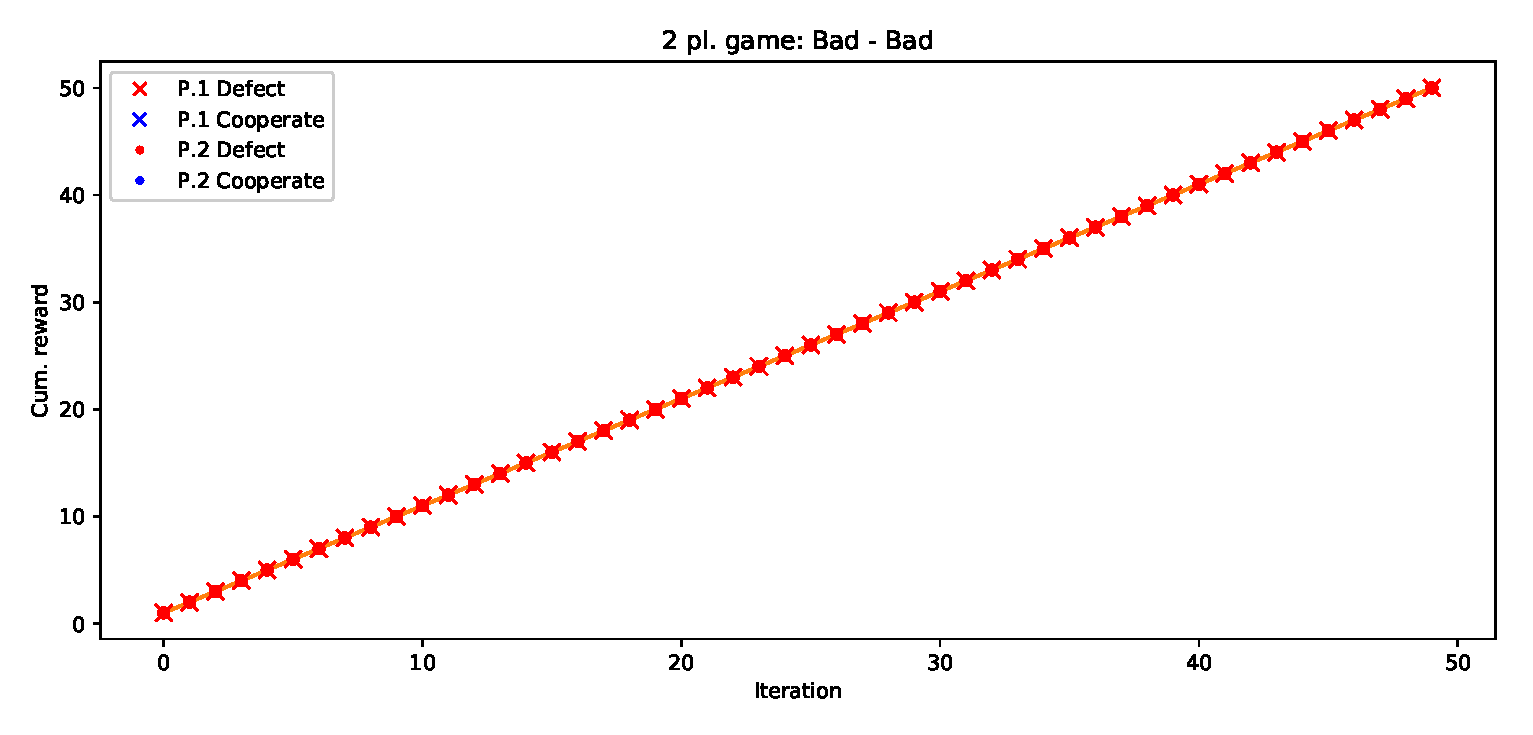
\includegraphics[width=1\columnwidth]{../img/ipd2p/ipd2p-rewards-Bad-Bad}
    \caption{Bad vs Bad}
    \label{fig:badvsbad}
\end{figure}

\begin{figure}[!ht]
    \centering
    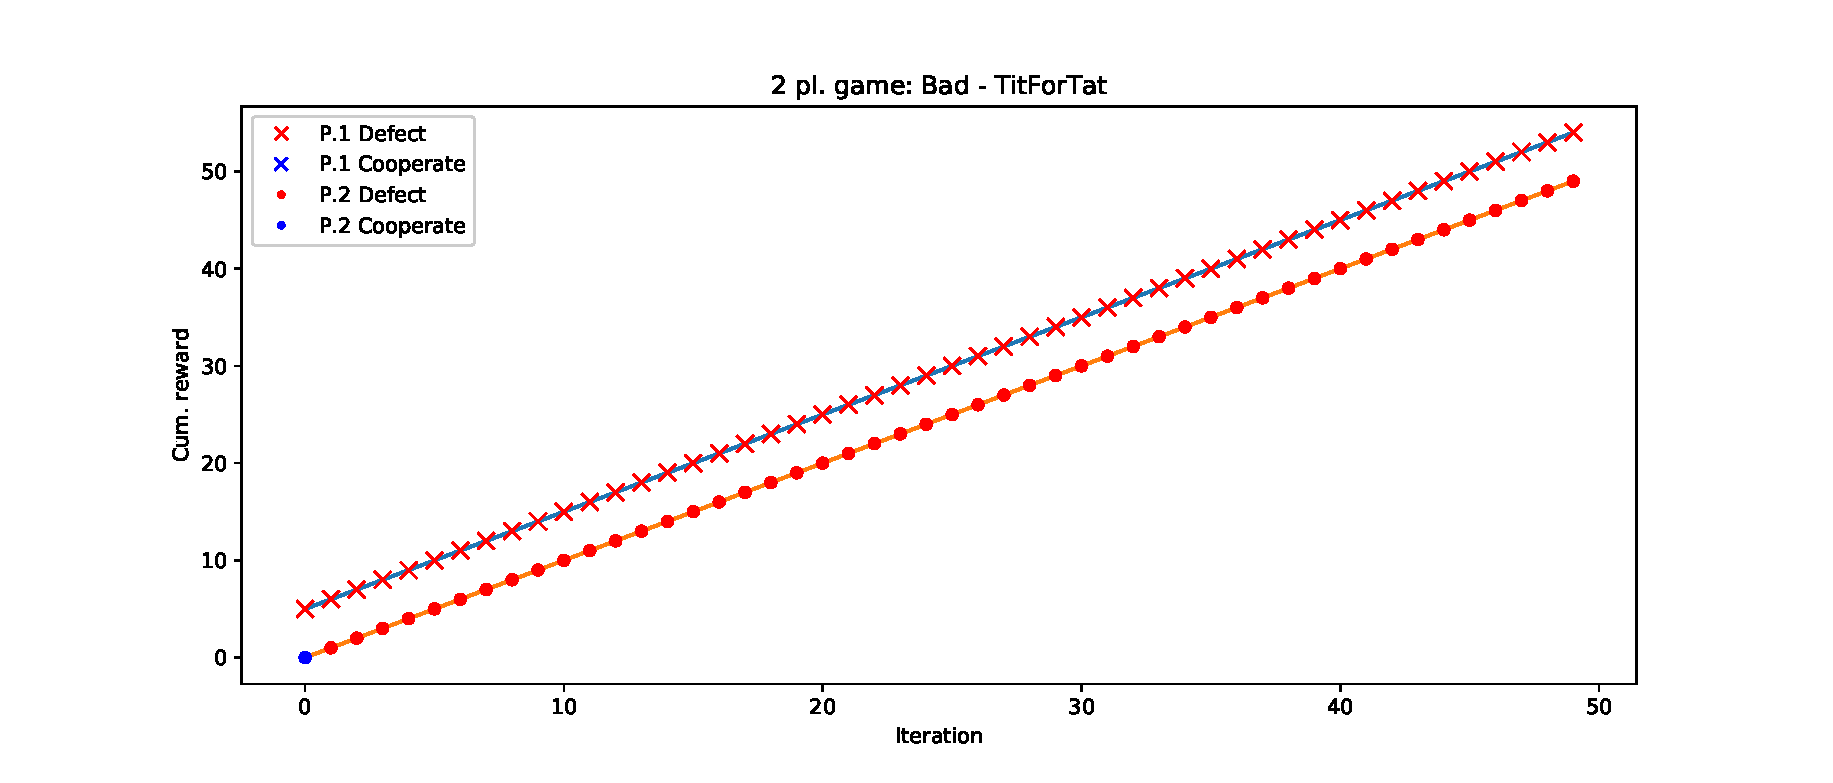
\includegraphics[width=1\columnwidth]{../img/ipd2p/ipd2p-rewards-Bad-TitForTat}
    \caption{Bad vs TfT}
    \label{fig:badvstft}
\end{figure}

\begin{figure}[!ht]
    \centering
    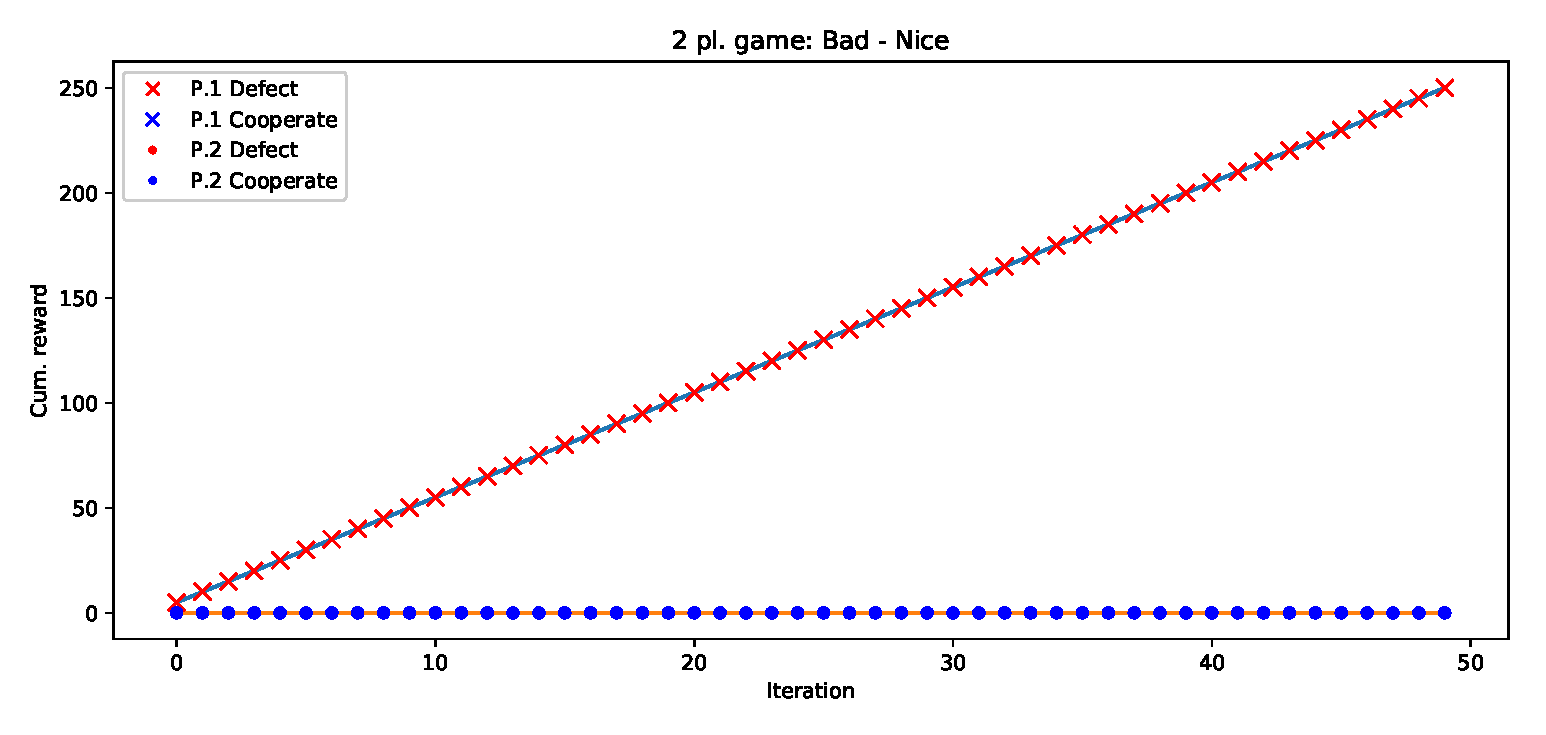
\includegraphics[width=1\columnwidth]{../img/ipd2p/ipd2p-rewards-Bad-Nice}
    \caption{Bad vs Nice}
    \label{fig:badvsnice}
\end{figure}

\begin{figure}[!ht]
    \centering
    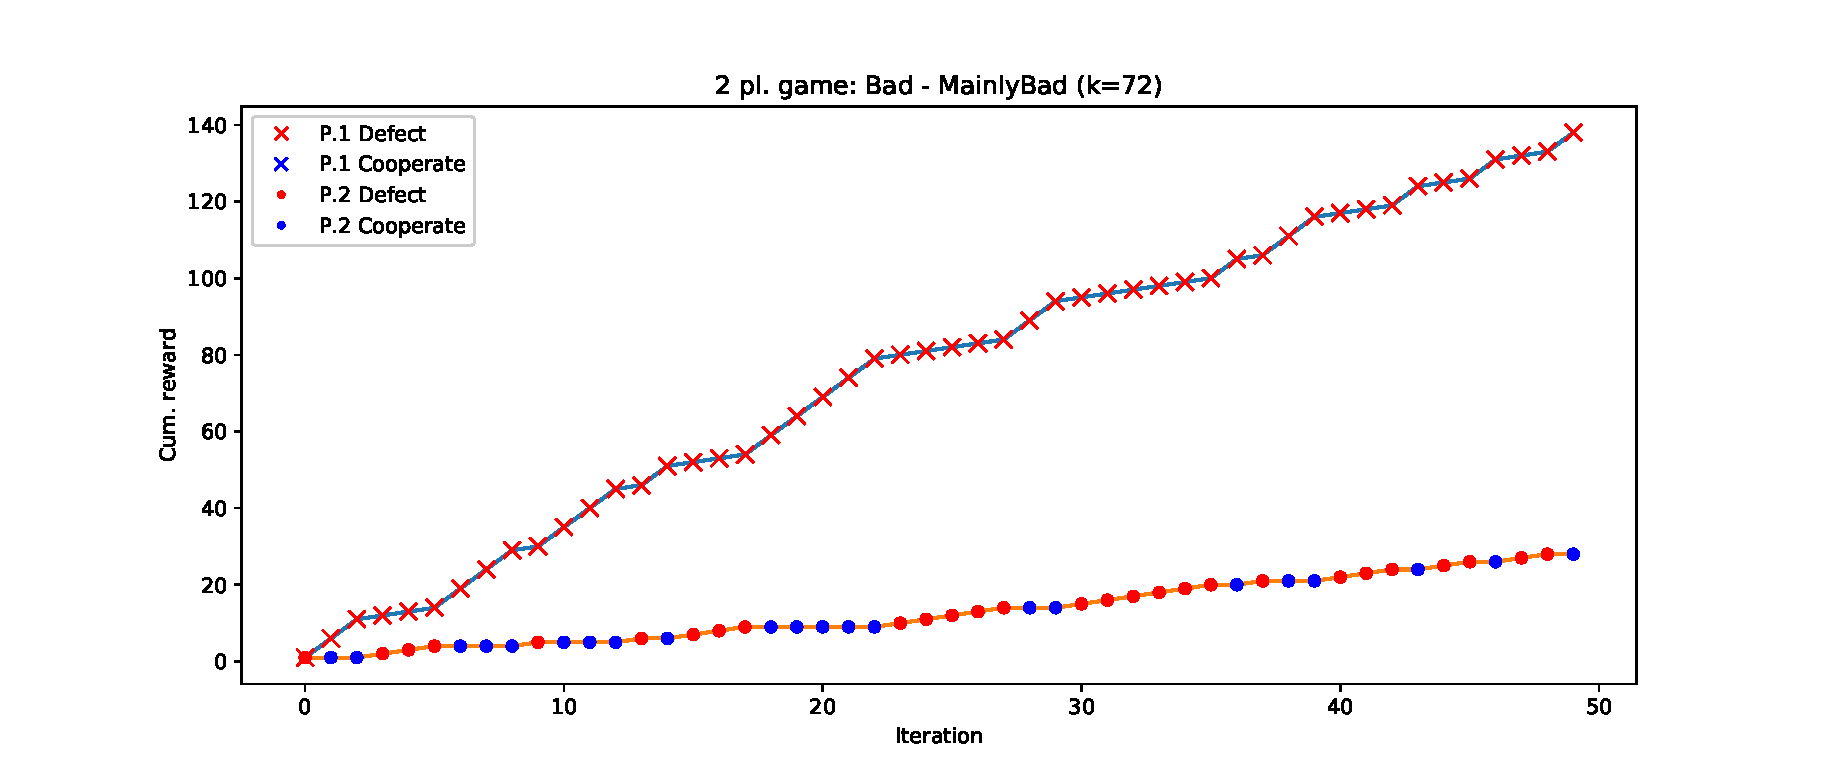
\includegraphics[width=1\columnwidth]{../img/ipd2p/ipd2p-rewards-Bad-MainlyBad(k=72)}
    \caption{Bad vs Mainly bad}
    \label{fig:badvsmainlybad}
\end{figure}

If we take a closer look, the combination of \textit{Nice} and one between \textit{TfT} or \textit{Nice} leads to better payoffs at the end of the runs as in Figures~[\ref{fig:tftvsindiff},\ref{fig:nicevsnice},\ref{fig:nicevstft}]. The idea behind this is that both players are getting the highest reward, not just one of them, and these choices are better compared to the \textit{Bad}-\textit{Nice} combination.
These are isolated cases that we are considering just because it is a study case, since the only strategy that wins against all the others and draws against itself is the \textit{Bad} one and so this is the strategy a smart player should choose, reminding both players have \textit{common knowledge}.

\begin{figure}[!ht]
    \centering
    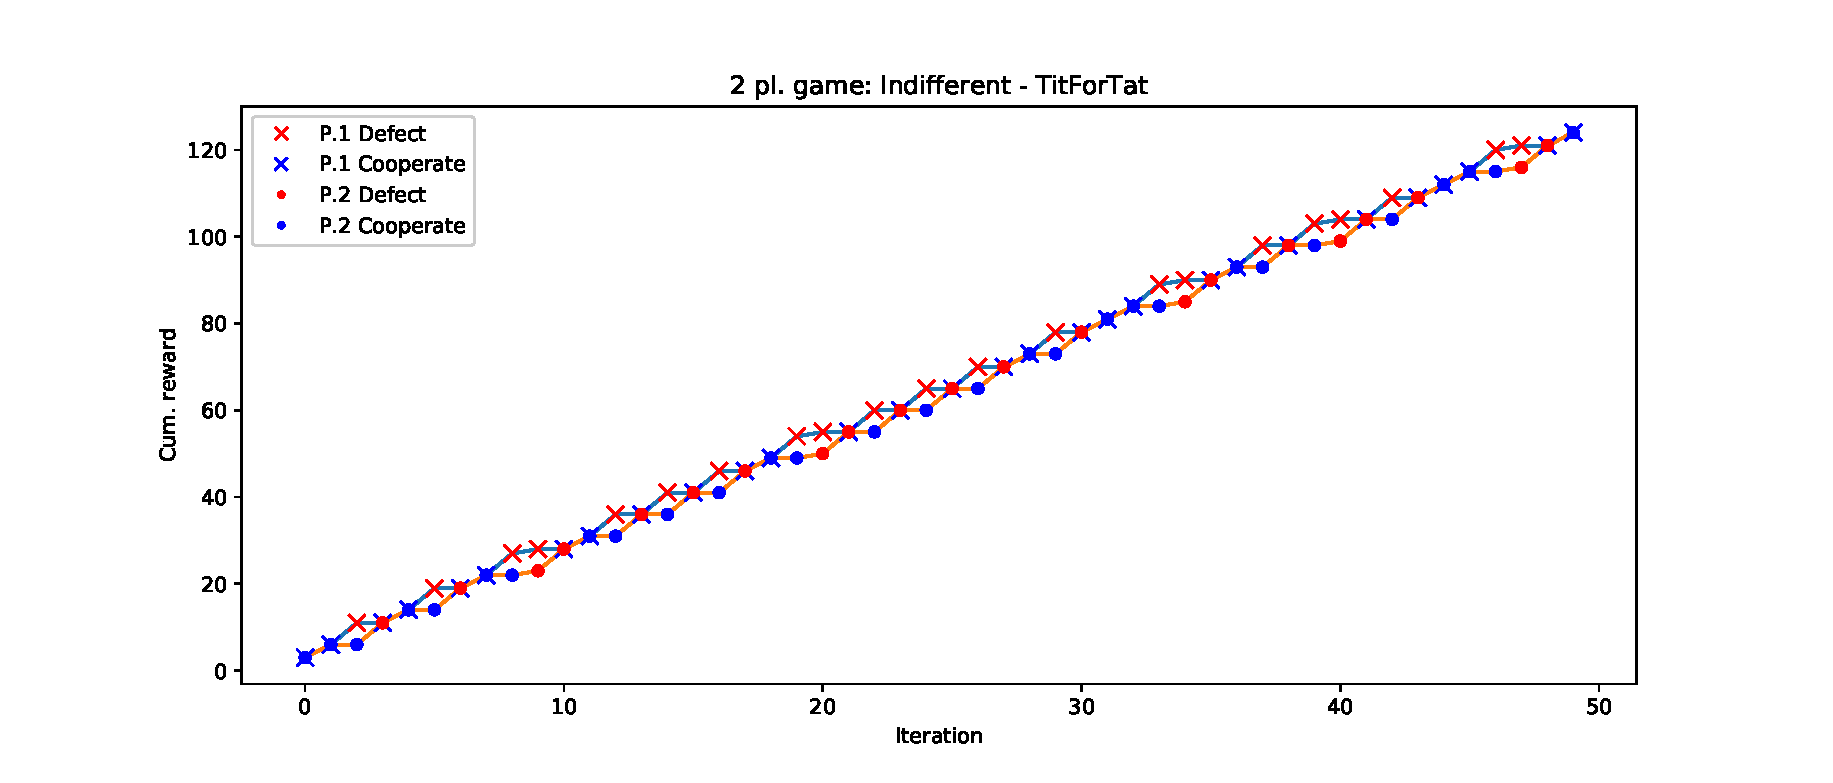
\includegraphics[width=1\columnwidth]{../img/ipd2p/ipd2p-rewards-Indifferent-TitForTat}
    \caption{TfT vs Indifferent}
    \label{fig:tftvsindiff}
\end{figure}

\begin{figure}[!ht]
    \centering
    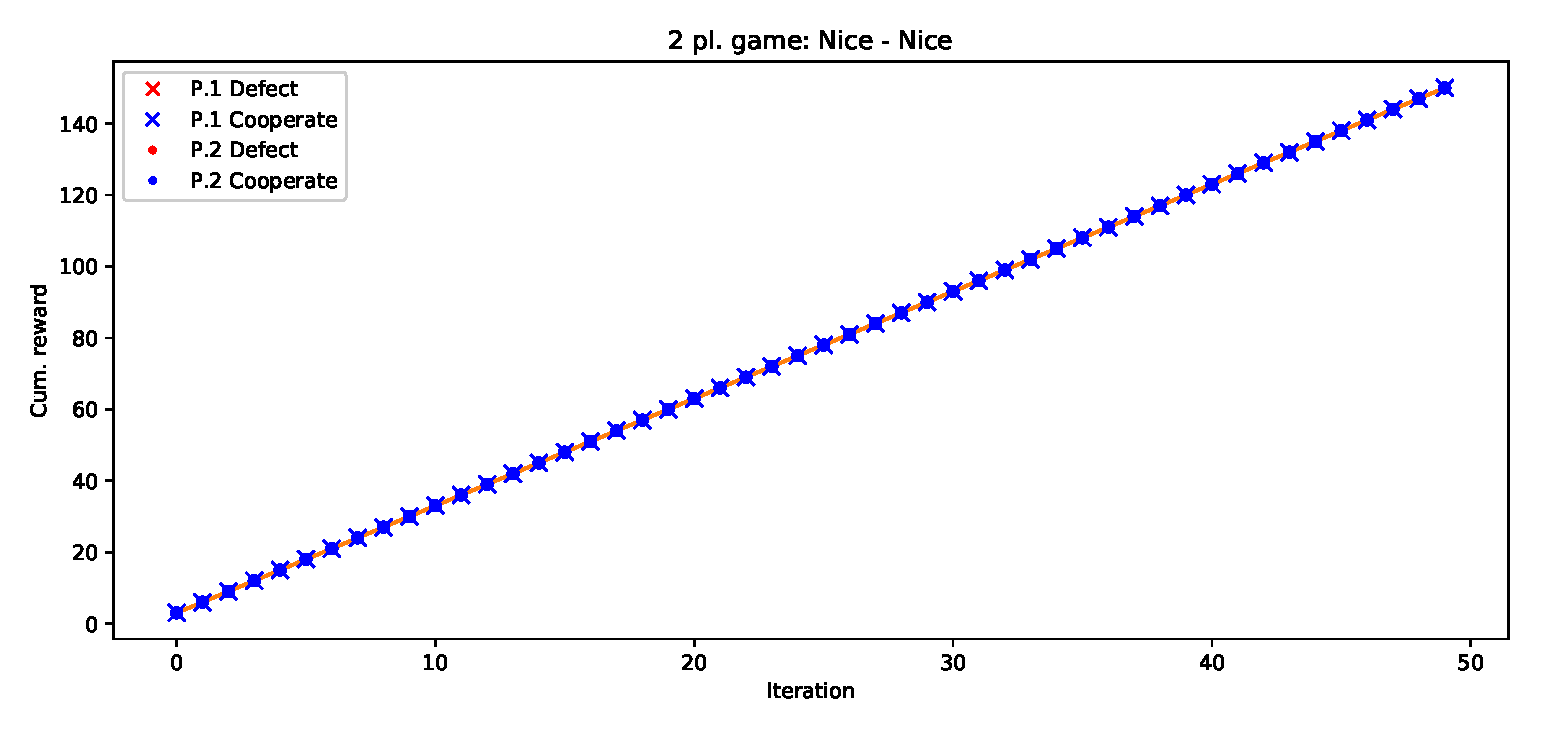
\includegraphics[width=1\columnwidth]{../img/ipd2p/ipd2p-rewards-Nice-Nice}
    \caption{Nice vs Nice}
    \label{fig:nicevsnice}
\end{figure}

\begin{figure}[!ht]
    \centering
    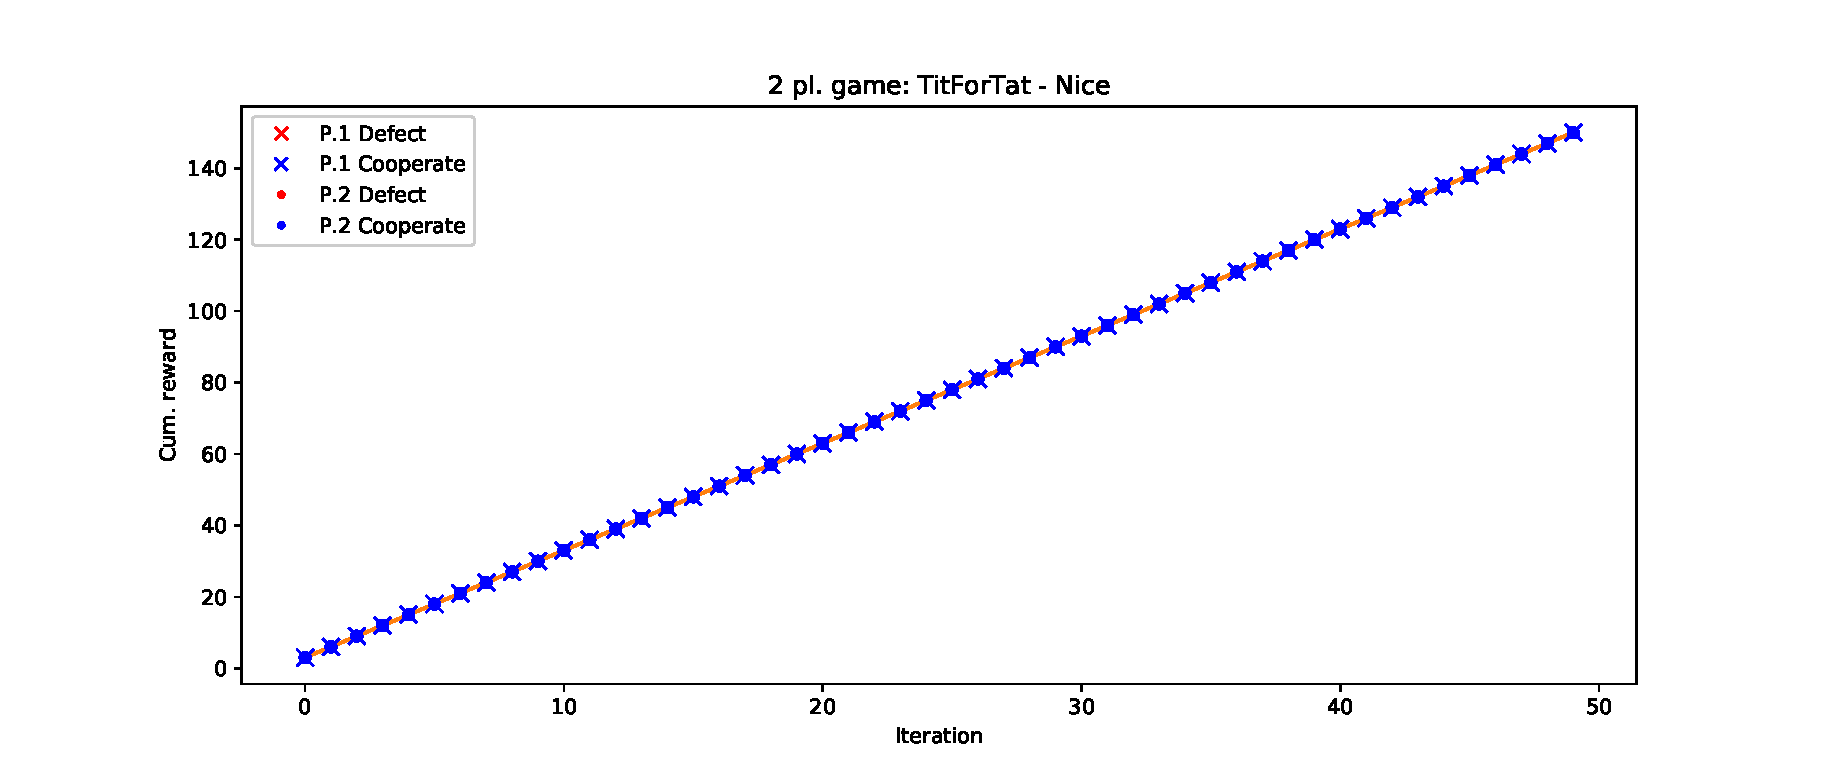
\includegraphics[width=1\columnwidth]{../img/ipd2p/ipd2p-rewards-TitForTat-Nice}
    \caption{Nice vs TfT}
    \label{fig:nicevstft}
\end{figure}

\begin{figure}[!ht]
    \centering
    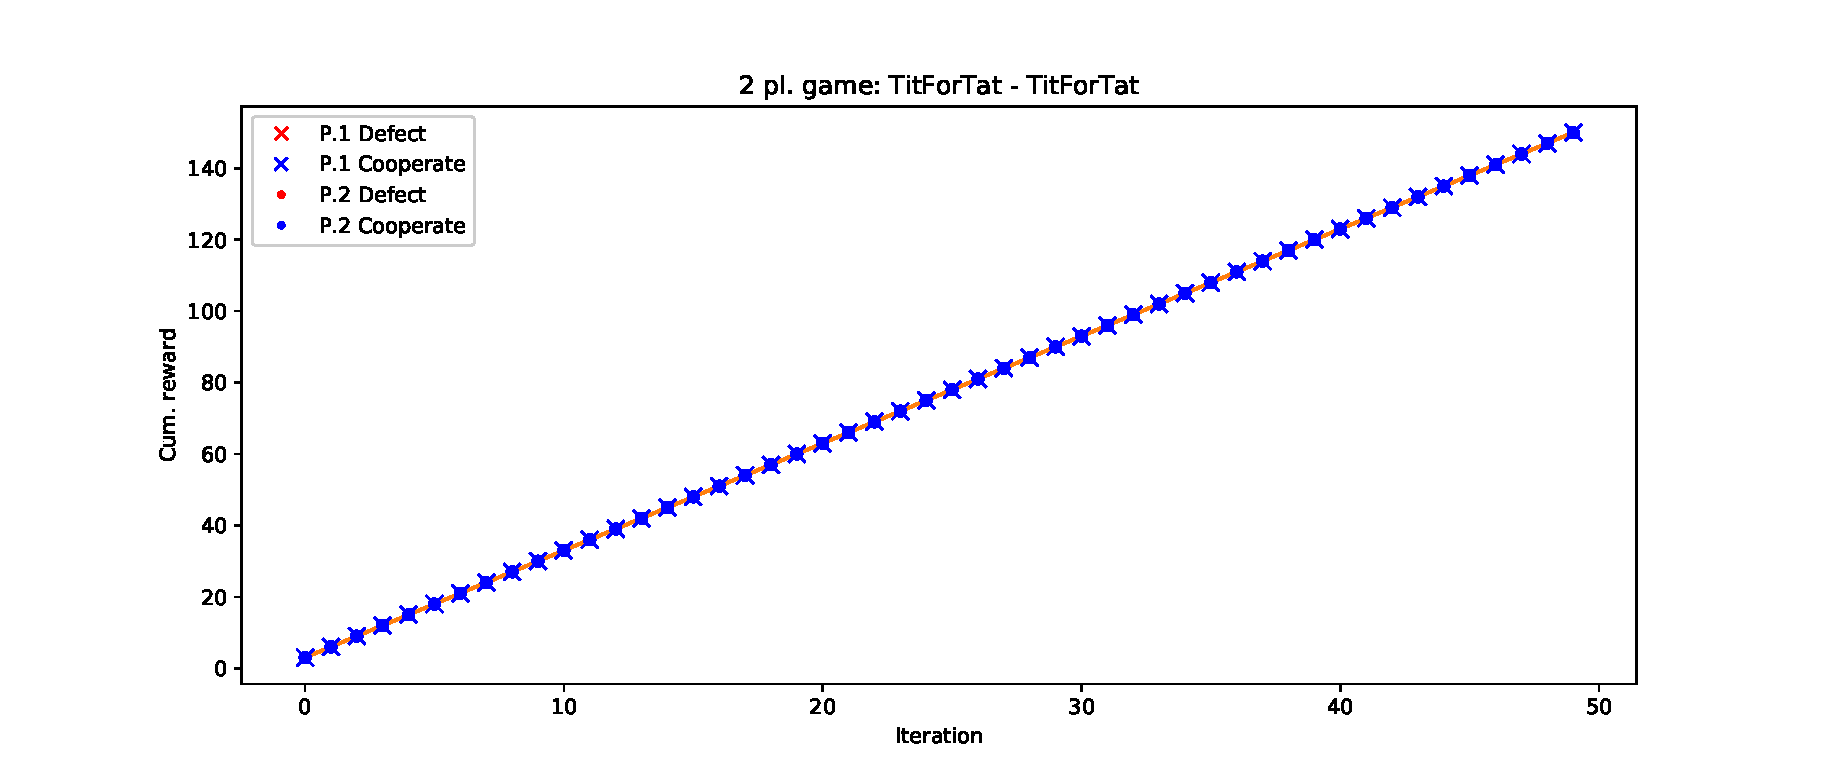
\includegraphics[width=1\columnwidth]{../img/ipd2p/ipd2p-rewards-TitForTat-TitForTat}
    \caption{TfT vs TfT}
    \label{fig:tftvstft}
\end{figure}

The \textit{TfT} strategy is interesting, because \textit{TfT} leads to almost the same cumulative reward as the opponent, and it is highly adaptive, even if fast-forgiving if it goes against a mainly bad strategy.
Or, in other words, \textit{TfT} is robust because it never defects first and never takes advantage for more than one iteration at a time.~\cite{fogelEvolvingBehaviors}
\textit{TfT} was also reported to be the winner over all the strategies analyzed by Axelrod in his extensive tests based on tournaments and evolutionary competition on the IPD, thoroughly described in~\cite{axelrod1981evolution,axelrod1984evolution} and taken up in~\cite{mathieu2017}.
The strategy was proposed to him by Anatol Rapoport.
A player might choose this move if he/she wants almost the same reward as the opponent. This strategy is even more interesting in the following sections.

In addition to these considerations simulations were performed multiple times to get insights of the mean and variance of the rewards that rule these games. Obviously the static strategies (as the \textit{Nice-Nice}, \autoref{fig:boxnn}), or the non-triggering ones, or the the ones without variations have a constant mean and $0$ std. On the other hand, it is interesting to notice that random strategies have a non null variance as shown in \textit{Mainly Bad-TitForTat}, \autoref{fig:boxmbvtft}. Anyway this does not imply that \textit{TitForTat} could ever win against such a strategy, it is only pointing out that there is a variation on subsequent runs based on the randomness of at least one of the two players: the \textit{TfT} strategy is a reactive strategy so it will be always ``late'', meaning that a player applying it will have always at most the same points of the opponent at the end of the game.

\begin{figure}[!ht]
    \centering
    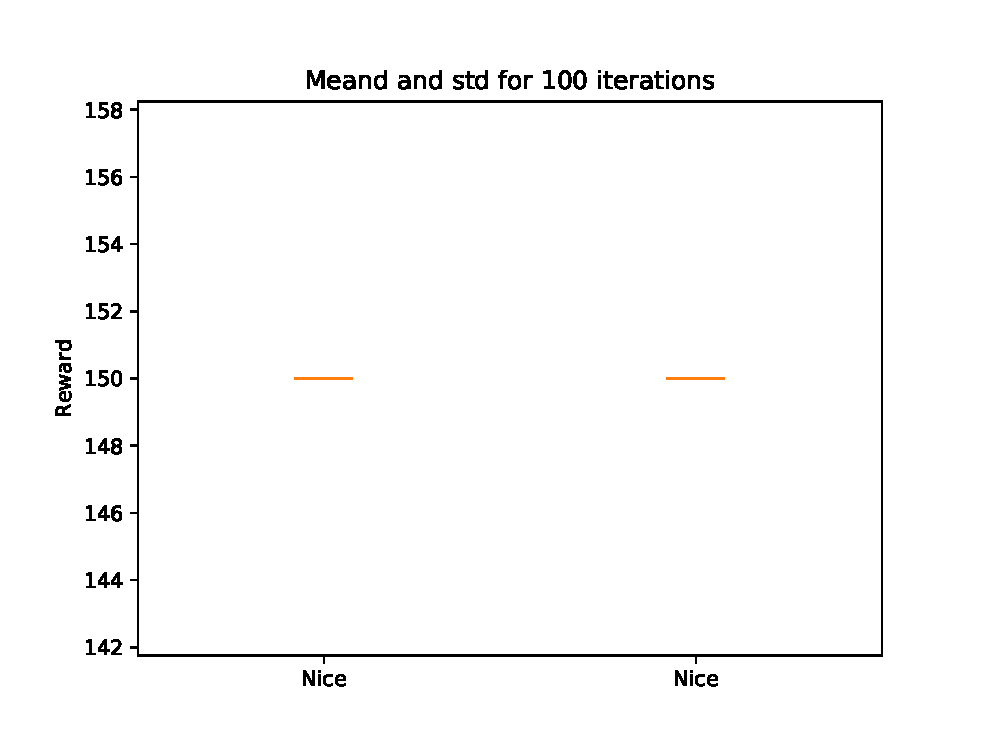
\includegraphics[width=1\columnwidth]{../img/ipd2p/ipd2p-boxplot-Nice-Nice}
    \caption{Nice vs Nice}
    \label{fig:boxnn}
\end{figure}

\begin{figure}[!ht]
    \centering
    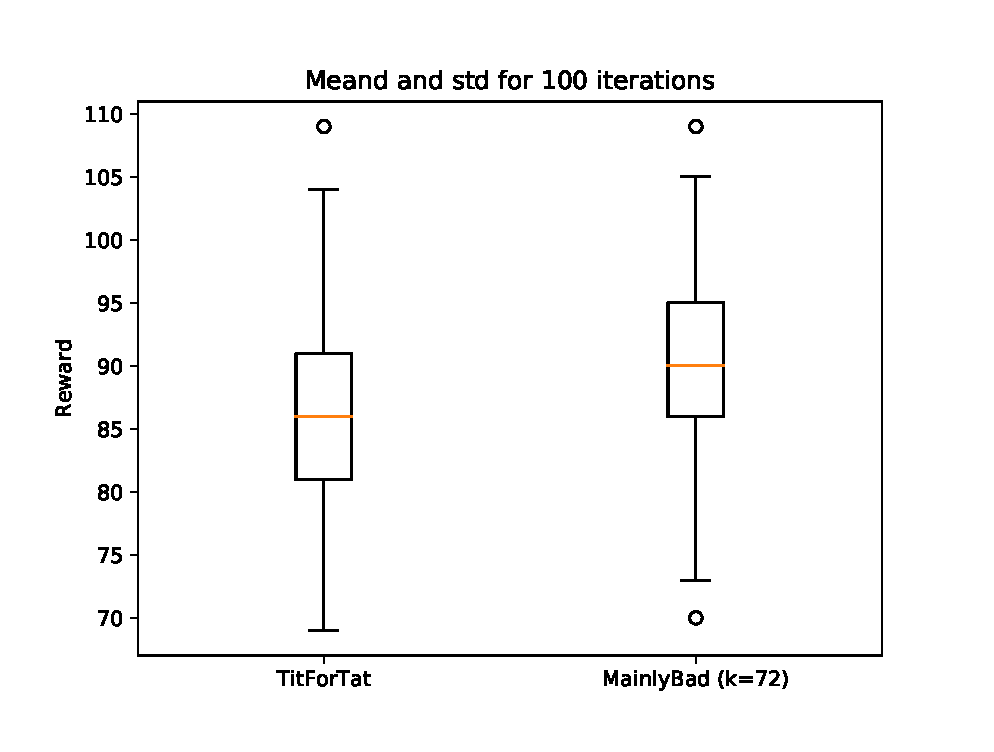
\includegraphics[width=1\columnwidth]{../img/ipd2p/ipd2p-boxplot-TitForTat-MainlyBad(k=72)}
    \caption{TfT vs Mainly Bad}
    \label{fig:boxmbvtft}
\end{figure}

More insights about this part, including the complete collection of the generated pictures, can be found in the repository and in \autoref{tab:ipd2p}, where collected statistics are presented\footnote{~For compactness, strategies in the tables of this paper are abbreviated with their short names. The $k$ value, if needed, is in parenthesis.}. Furthermore, we can see that the only strategies that reach $0$ as a final payoff are the \textit{Nice} ones, while the \textit{TfT, Tf2T, GrT, Bad} have a higher minimum value.

In the end, it is impossible to make the optimal score against all strategies. The most intuitive reason is a consequence of the first move: to play optimally against a \textit{Bad} guy it is necessary to defect at the first round, to play optimally against \textit{GrT} it is necessary to cooperate until the last round where you should defect.~\cite{mathieu2017}
But the number of rounds is unknown to the players and they should know in advance the type of the opponent: this would allow them to adapt their strategy, but this is not possible based on the rules of the game. 

\section{Multiple players IPD - Round-robin scheme} \label{s:IPDMP}
The IPD with \textit{round-robin} (RR) scheme, used to match-up the opponents, consists in a number of players, with multiple strategies, not necessarily different, with each player playing once against each other for a \texttt{NUM\_ITER = 50} of times.

Each player chooses its fixed strategy at the beginning of the tournament and holds it throughout the course of the whole tournament. Nobody knows the strategies of the other players.

In short, it is a variation of the previous case, in which multiple players, with possibly different strategies, play in a RR way. The variation consists in the fact that a single player will win the tournament if at the end of it he has the highest cumulative payoff.

Tournament statistics, like points and counts of cooperation and defection moves, along with the percentage of cooperation, are shown in \autoref{tab:ipdmp}.

\begin{table}[ht]
    \caption{50-players IPD, sorted by points, statistics}
    \label{tab:ipdmp}
    \centering
    \begin{tabular}{lrrrrrrr} \toprule
    	         & \multicolumn{2}{c}{Points} & \multicolumn{2}{c}{Coop. count} & \multicolumn{2}{c}{Defect count} & \\
    	Strategy &      avg &   std &      avg &   std &      avg &   std &   C \% \\ \midrule
    	    Nice &   4948.5 & 38.81 &   2450.0 &  0.00 &      0.0 &  0.00 &   100 \\
    	    Nice &   4926.0 & 43.24 &   2450.0 &  0.00 &      0.0 &  0.00 &   100 \\
    	     TfT &   5884.6 & 26.69 &   1664.8 & 10.76 &    785.2 & 10.76 &    68 \\
    	 MB (81) &   5411.3 & 65.52 &    459.6 & 19.84 &   1990.4 & 19.84 &    19 \\
    	 MB (70) &   5387.1 & 62.40 &    728.7 & 17.36 &   1721.3 & 17.36 &    30 \\
    	 MB (85) &   5422.8 & 58.42 &    373.9 & 17.92 &   2076.1 & 17.92 &    15 \\
    	    Nice &   4206.6 & 46.10 &   2450.0 &  0.00 &      0.0 &  0.00 &   100 \\
    	     Ind &   5246.0 & 66.33 &   1221.6 & 15.01 &   1228.4 & 15.01 &    50 \\
    	  MN (8) &   4396.3 & 43.95 &   2260.2 & 10.91 &    189.8 & 10.91 &    92 \\
    	    Tf2T &   5136.4 & 34.72 &   1589.9 & 19.76 &    860.1 & 19.76 &    65 \\
    	     Ind &   5222.4 & 66.27 &   1220.1 & 32.81 &   1229.9 & 32.81 &    50 \\
    	     GrT &   5231.7 & 89.53 &    196.1 &  0.32 &   2253.9 &  0.32 &     8 \\
    	     Ind &   5223.1 & 62.10 &   1217.9 & 29.42 &   1232.1 & 29.42 &    50 \\
    	     Ind &   5258.2 & 90.87 &   1218.6 & 28.88 &   1231.4 & 28.88 &    50 \\
    	 MN (17) &   4651.7 & 68.18 &   2033.3 & 20.59 &    416.7 & 20.59 &    83 \\
    	     Ind &   5216.1 & 82.14 &   1223.4 & 26.90 &   1226.6 & 26.90 &    50 \\
    	     Bad &   5362.4 & 78.10 &      0.0 &  0.00 &   2450.0 &  0.00 &     0 \\
    	    Nice &   4207.5 & 42.83 &   2450.0 &  0.00 &      0.0 &  0.00 &   100 \\
    	    Nice &   4205.1 & 32.53 &   2450.0 &  0.00 &      0.0 &  0.00 &   100 \\
    	 MB (78) &   5449.6 & 39.35 &    545.4 & 22.11 &   1904.6 & 22.11 &    22 \\
    	    Tf2T &   5136.4 & 18.00 &   1590.7 &  8.56 &    859.3 &  8.56 &    65 \\
    	     TfT &   5383.9 & 32.66 &   1420.8 & 13.31 &   1029.2 & 13.31 &    58 \\
    	    Tf2T &   5139.4 & 18.24 &   1598.6 & 18.54 &    851.4 & 18.54 &    65 \\
    	     Ind &   5247.8 & 88.62 &   1219.9 & 21.74 &   1230.1 & 21.74 &    50 \\
    	    Nice &   4208.7 & 28.55 &   2450.0 &  0.00 &      0.0 &  0.00 &   100 \\
    	     TfT &   5386.4 & 26.80 &   1425.1 & 11.69 &   1024.9 & 11.69 &    58 \\
    	     Bad &   5343.2 & 41.91 &      0.0 &  0.00 &   2450.0 &  0.00 &     0 \\
    	     GrT &   5213.7 & 42.01 &    196.2 &  0.63 &   2253.8 &  0.63 &     8 \\
    	  MN (3) &   4278.4 & 28.71 &   2379.4 &  9.16 &     70.6 &  9.16 &    97 \\
    	     Ind &   5226.7 & 48.77 &   1222.9 & 21.45 &   1227.1 & 21.45 &    50 \\
    	     TfT &   5367.2 & 22.34 &   1414.7 &  9.78 &   1035.3 &  9.78 &    58 \\
    	    Tf2T &   5144.3 & 18.15 &   1599.4 & 11.92 &    850.6 & 11.92 &    65 \\
    	    Tf2T &   5121.5 & 29.34 &   1582.2 & 17.42 &    867.8 & 17.42 &    65 \\
    	 MB (97) &   5386.9 & 65.11 &     74.5 &  6.52 &   2375.5 &  6.52 &     3 \\
    	     Bad &   5359.2 & 41.10 &      0.0 &  0.00 &   2450.0 &  0.00 &     0 \\
    	     GrT &   5192.0 & 45.06 &    196.4 &  0.97 &   2253.6 &  0.97 &     8 \\
    	     GrT &   5185.0 & 62.03 &    196.7 &  1.16 &   2253.3 &  1.16 &     8 \\
    	     TfT &   5385.2 & 34.27 &   1422.7 & 14.85 &   1027.3 & 14.85 &    58 \\
    	    Tf2T &   5137.9 & 22.20 &   1586.5 & 14.67 &    863.5 & 14.67 &    65 \\
    	    Tf2T &   5148.6 & 16.61 &   1594.7 & 10.07 &    855.3 & 10.07 &    65 \\
    	     TfT &   5366.2 & 27.54 &   1415.7 & 10.52 &   1034.3 & 10.52 &    58 \\
    	     TfT &   5387.7 & 27.79 &   1422.7 & 14.49 &   1027.3 & 14.49 &    58 \\
    	     TfT &   5380.6 & 32.89 &   1421.3 & 13.60 &   1028.7 & 13.60 &    58 \\
    	 MB (81) &   5412.9 & 61.21 &    469.9 & 15.43 &   1980.1 & 15.43 &    19 \\
    	     Bad &   5330.8 & 33.93 &      0.0 &  0.00 &   2450.0 &  0.00 &     0 \\
    	 MB (99) &   5379.4 & 61.92 &     26.3 &  5.77 &   2423.7 &  5.77 &     1 \\
    	     Bad &   5322.0 & 21.00 &      0.0 &  0.00 &   2450.0 &  0.00 &     0 \\
    	     GrT &   5223.5 & 79.12 &    196.1 &  0.32 &   2253.9 &  0.32 &     8 \\
    	 MN (42) &   5110.5 & 70.63 &   1421.1 & 25.18 &   1028.9 & 25.18 &    58 \\
    	 MB (98) &   5352.7 & 35.40 &     48.7 &  5.46 &   2401.3 &  5.46 &     2 \\ \bottomrule
    \end{tabular}
\end{table}

% python ipdmp.py --saveimg --nplay 8 --latex
\textbf{REPLACE TABLES, UNSORTED}
\begin{table}[ht]
    \caption{8-players IPD, sorted by points, statistics}
    \label{tab:ipdmp8}
    \centering
	\begin{tabular}{lrrrrrrrr}
		\toprule
		         & \multicolumn{2}{c}{Points} &        & \multicolumn{2}{c}{Coop. count} & \multicolumn{2}{c}{Defect count} &        \\
		Strategy &   avg &                std &  yield &   avg &                     std &   avg &                      std &   C \% \\
		\midrule
		Bad      & 874.0 &              29.51 & 100.00 &   0.0 &                    0.00 & 350.0 &                     0.00 &   0.00 \\
		Tf2T     & 680.5 &              16.99 &  71.16 & 213.5 &                    9.11 & 136.5 &                     9.11 &  61.00 \\
		GrT      & 850.3 &              31.69 &  98.28 &   7.0 &                    0.00 & 343.0 &                     0.00 &   2.00 \\
		Ind      & 740.6 &              15.43 &  68.23 & 175.9 &                    5.43 & 174.1 &                     5.43 &  50.26 \\
		MN (27)  & 671.3 &              16.29 &  54.68 & 256.8 &                    8.98 &  93.2 &                     8.98 &  73.37 \\
		TfT      & 729.8 &              11.55 &  77.10 & 178.9 &                    5.59 & 171.1 &                     5.59 &  51.11 \\
		MB (72)  & 818.1 &              31.31 &  80.80 &  95.0 &                    6.46 & 255.0 &                     6.46 &  27.14 \\
		Nice     & 528.3 &              19.67 &  39.70 & 350.0 &                    0.00 &   0.0 &                     0.00 & 100.00 \\
		\bottomrule
	\end{tabular}
\end{table}

\begin{figure}[!ht]
    \centering
    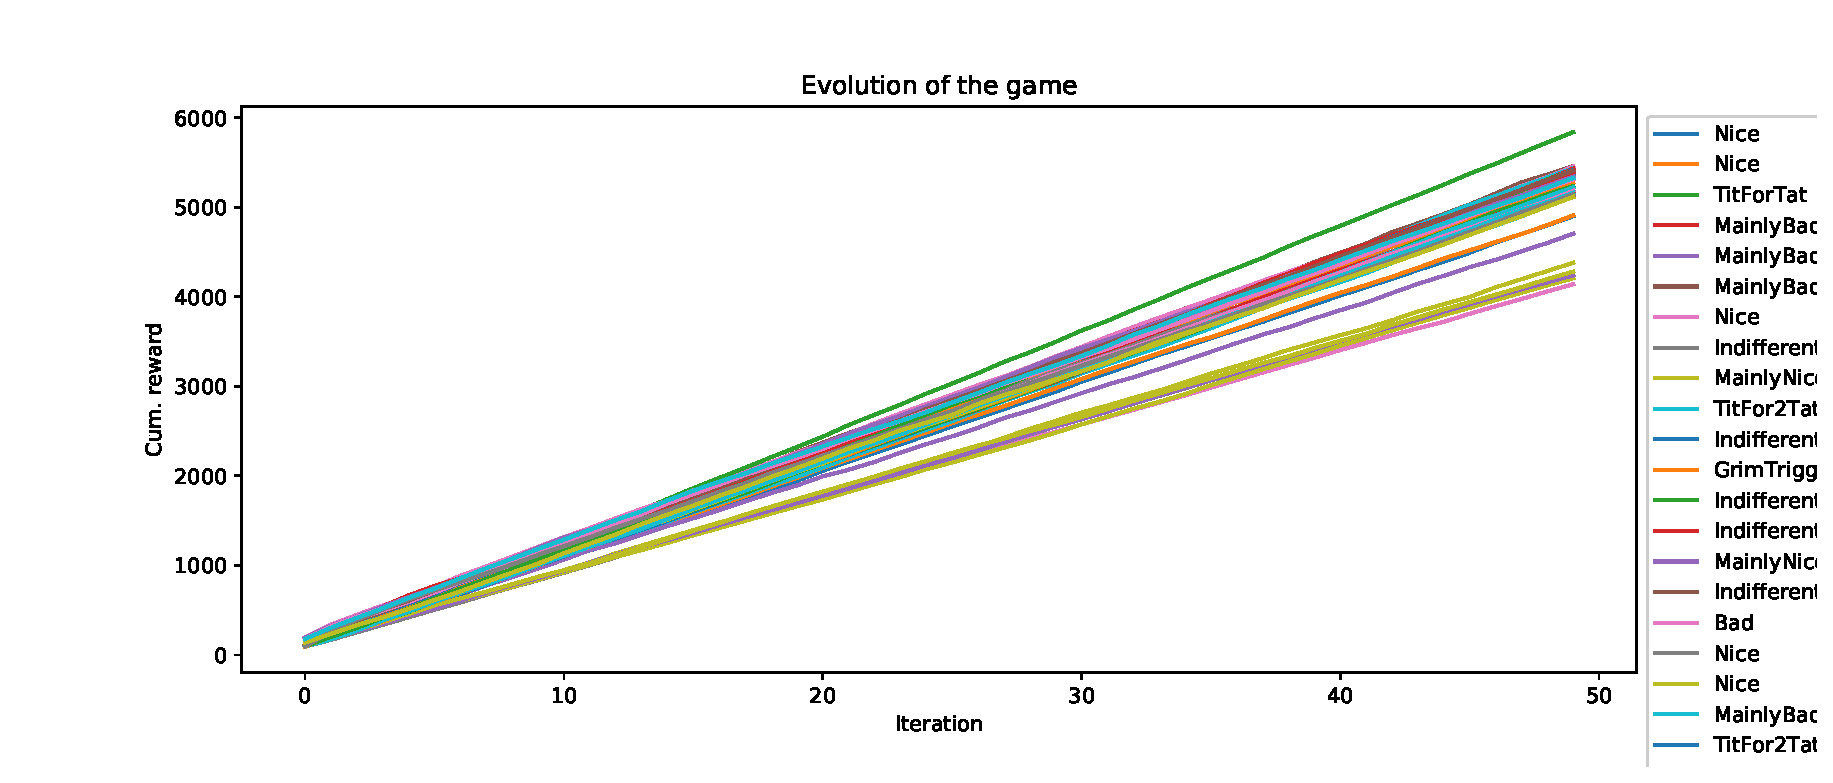
\includegraphics[width=1\columnwidth]{../img/ipdmp/ipdmp-evolution-of-game-50}
    \caption{Evolution of the game}
    \label{fig:boxIPDMPevo}
\end{figure}

\begin{figure}[!ht]
    \centering
    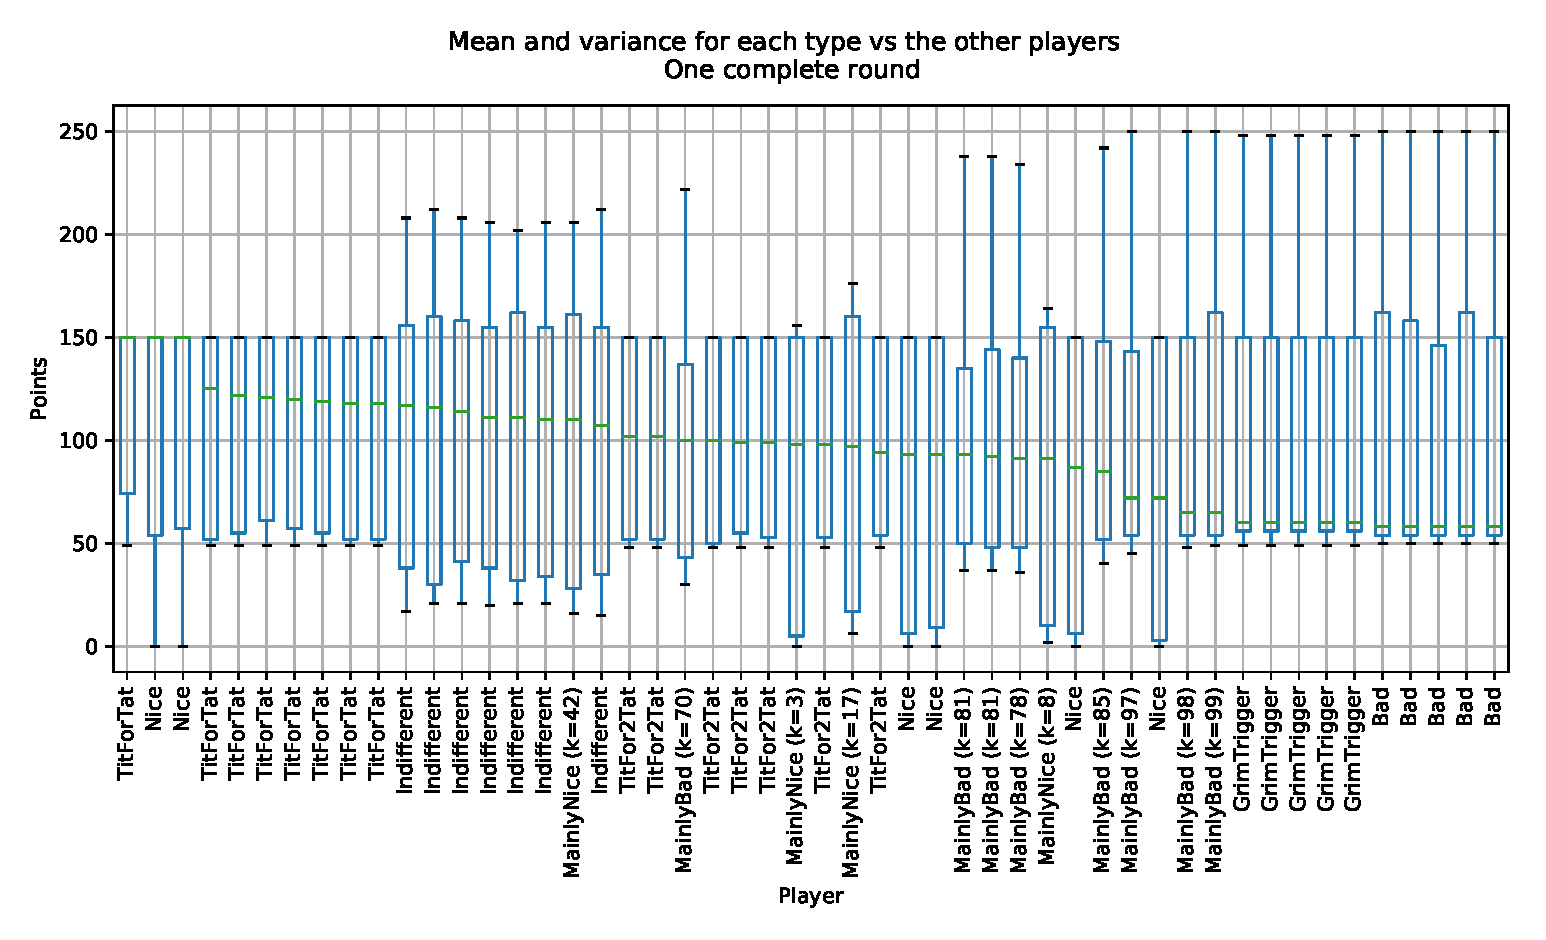
\includegraphics[width=1\columnwidth]{../img/ipdmp/ipdmp-boxplot-single-match-50}
    \caption{Boxplot of a single match}
    \label{fig:boxIPDMPsingle}
\end{figure}

\begin{figure}[!ht]
    \centering
    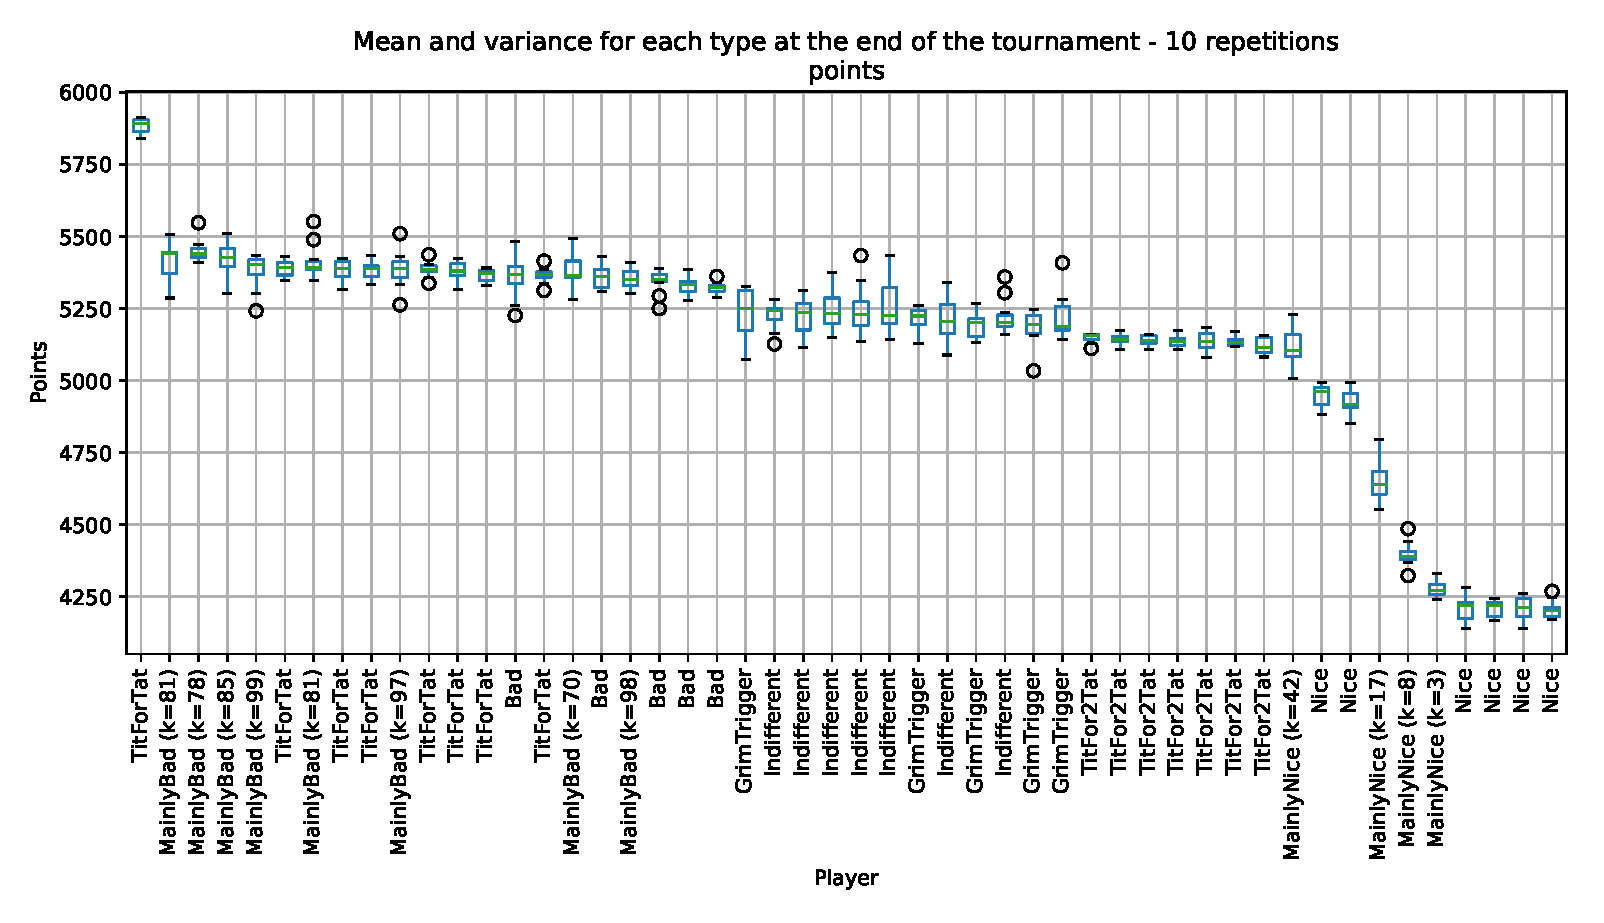
\includegraphics[width=1\columnwidth]{../img/ipdmp/ipdmp-boxplot-final-points-50}
    \caption{Boxplot of the final points}
    \label{fig:boxIPDMPfinal}
\end{figure}

The results of the tournament (and of the following study-cases) depend on the initial population and the balance between the amount of \textit{Bad} and \textit{TfT} players. The best strategy overall seems to be the \textit{TfT} one.
These outcomes may also be found in~\cite{mathieu2017}.

\textbf{ADD FIGURE of 8 players}
We can easily see that in a 8 players game (Figure \ref{fig:}) the best strategy overall is the \textit{Bad} one. We link this behaviour to a subtle balance between ``good'' and ``bad'' strategies: since \textit{TfT} as we have already seen is a reactive strategy to win a tournament it should be coupled with enough (mainly)good players otherwise the bad one will easily overcome and win the tournament. In the end we found out after various tries that a good setup is where we have more ``good'' strategies with respect to the bad ones to have a \textit{TfT} winner. We could not found this consideration in the literature, but we believe that is important and worth noticing even if this can be easily explained by the game's instrinsics. Notice this would help to interpret results and give them the right meaning. \textit{TfT} is \textit{not} the best strategy(even if we admit that such a strategy exists), but is the best strategy in some particular tournaments. Even though, surely, \textit{TfT} is one of the best strategies that helps to maximize the score.
% todo: explain why TfT is the best in our case

Similarly to what was pointed out previously, we can see variations of the results obtained by running the simulations multiple times and generating boxplots. 
Since we have introduced the random strategies, the result of a one-shot complete game may differ with respect to the average results; a simple example of this is the 8 players game where on average the \textit{Bad} guy wins but there may be runs where the \textit{GrT} strategy wins (as evidenced in \autoref{fig: da8}) 
% todo: say something about the specified population and who wins

\section{Repeated multiple players IPD - RR scheme} \label{s:rIPDMP}
The previuosly defined MPIPD round-robin scheme tournament was iterated many times to collect more advanced statistics.
We identify this schema as a \textit{Repeated multiple players IPD} (rMPIPD).

Two separated scenarios have been developed to study the behaviour of the populations and the convergence speed by simulations. A population is said to be converging if more than $3/4$ of it has the same strategy type at the end of a complete round. The base rules are the same as pointed out in the previous sections (\textit{common knowledge}, ...).

\subsection{Static Population}
In this case the number of players is fixed. Each player implements a strategy choosing it with equal probability from the strategies set. At the end of each round the first third of the population is doubled (the third that achieves the highest cumulative payoff), and the last third is removed. In this way we can ensure a static number of players and then study the convergence of the population through consecutive rounds.
Convergence is declared when more than $3/4$ of the players have their strategies of the same type, or when a maximum number of repetitions are reached.
This method also resembles how Axelrod made his tests~\cite[\S 2.6]{mathieu2017}~\cite{axelrod1984evolution}.

Figures~[\ref{fig:constR},\ref{fig:constFI},\ref{fig:constLI}] show the evolution of a population of 50 players over some iterations.
Details on the evolution of the population, grouped by strategy type, are presented in \autoref{tab:ripdmp-const}.
We can easily see how the \textit{TfT} strategy outpaces the others in a fast way: it requires only $4$ iterations for \textit{TfT} to overcome the other strategies.

\begin{figure}[!ht]
    \centering
    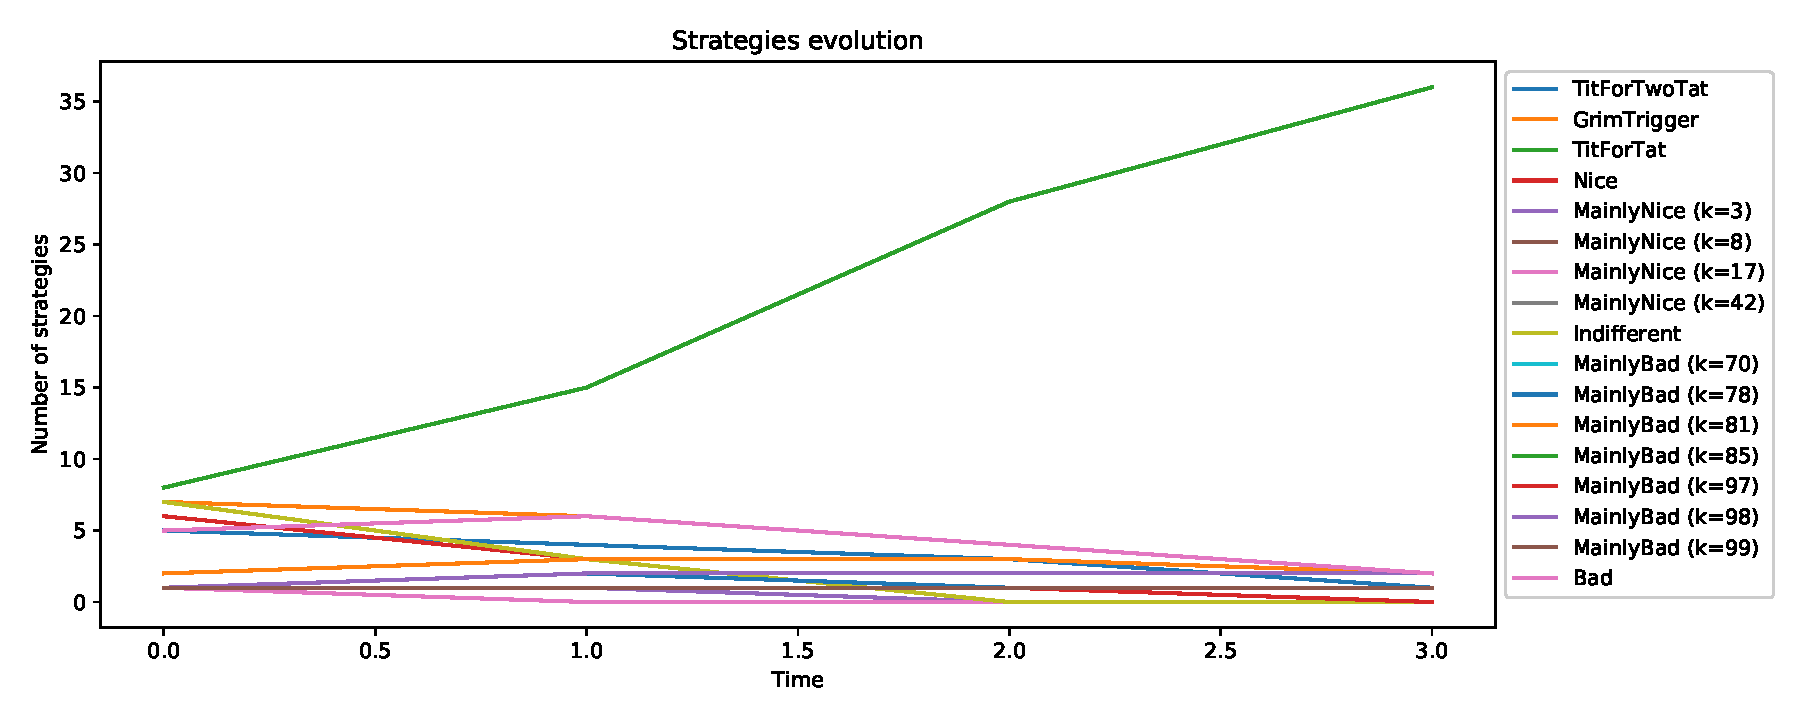
\includegraphics[width=1\columnwidth]{../img/ripdmp-const/ripdmp-evolution-const-pop-50}
    \caption{Evolution of rIPDMP, constant population of 50}
    \label{fig:constR}
\end{figure}

\begin{figure}[!ht]
    \centering
    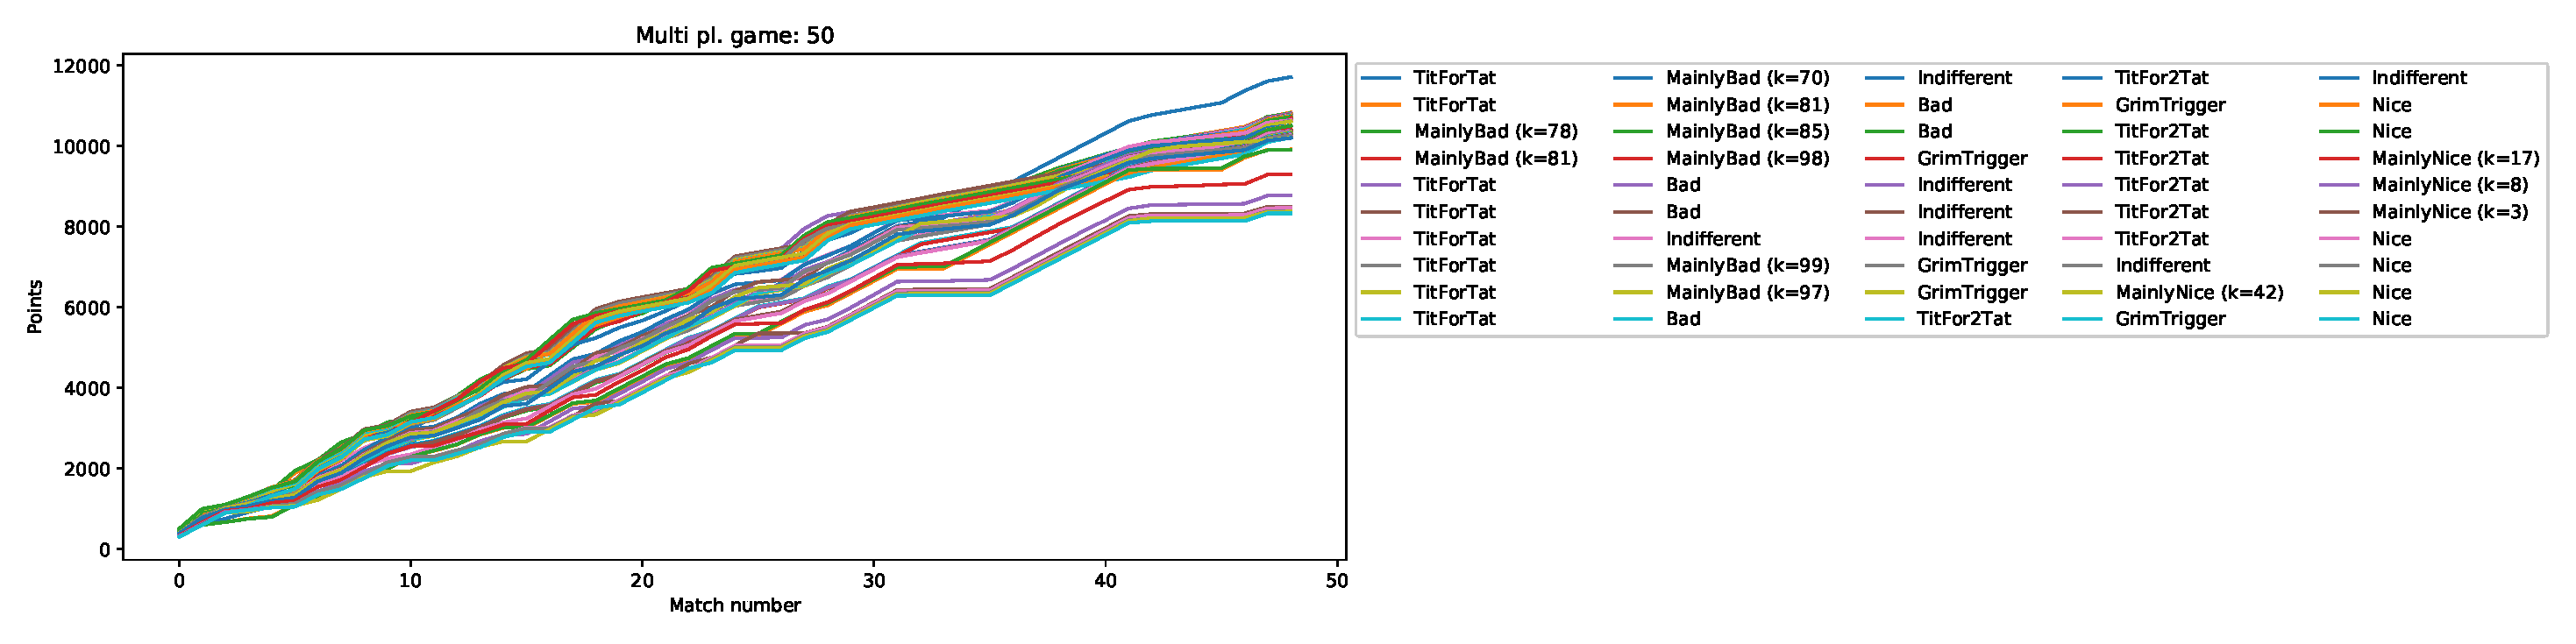
\includegraphics[width=1\columnwidth]{../img/ripdmp-const/ripdmp-scores-const-pop-50-r0}
    \caption{First iteration scores ($it=0$)}
    \label{fig:constFI}
\end{figure}

\begin{figure}[!ht]
    \centering
    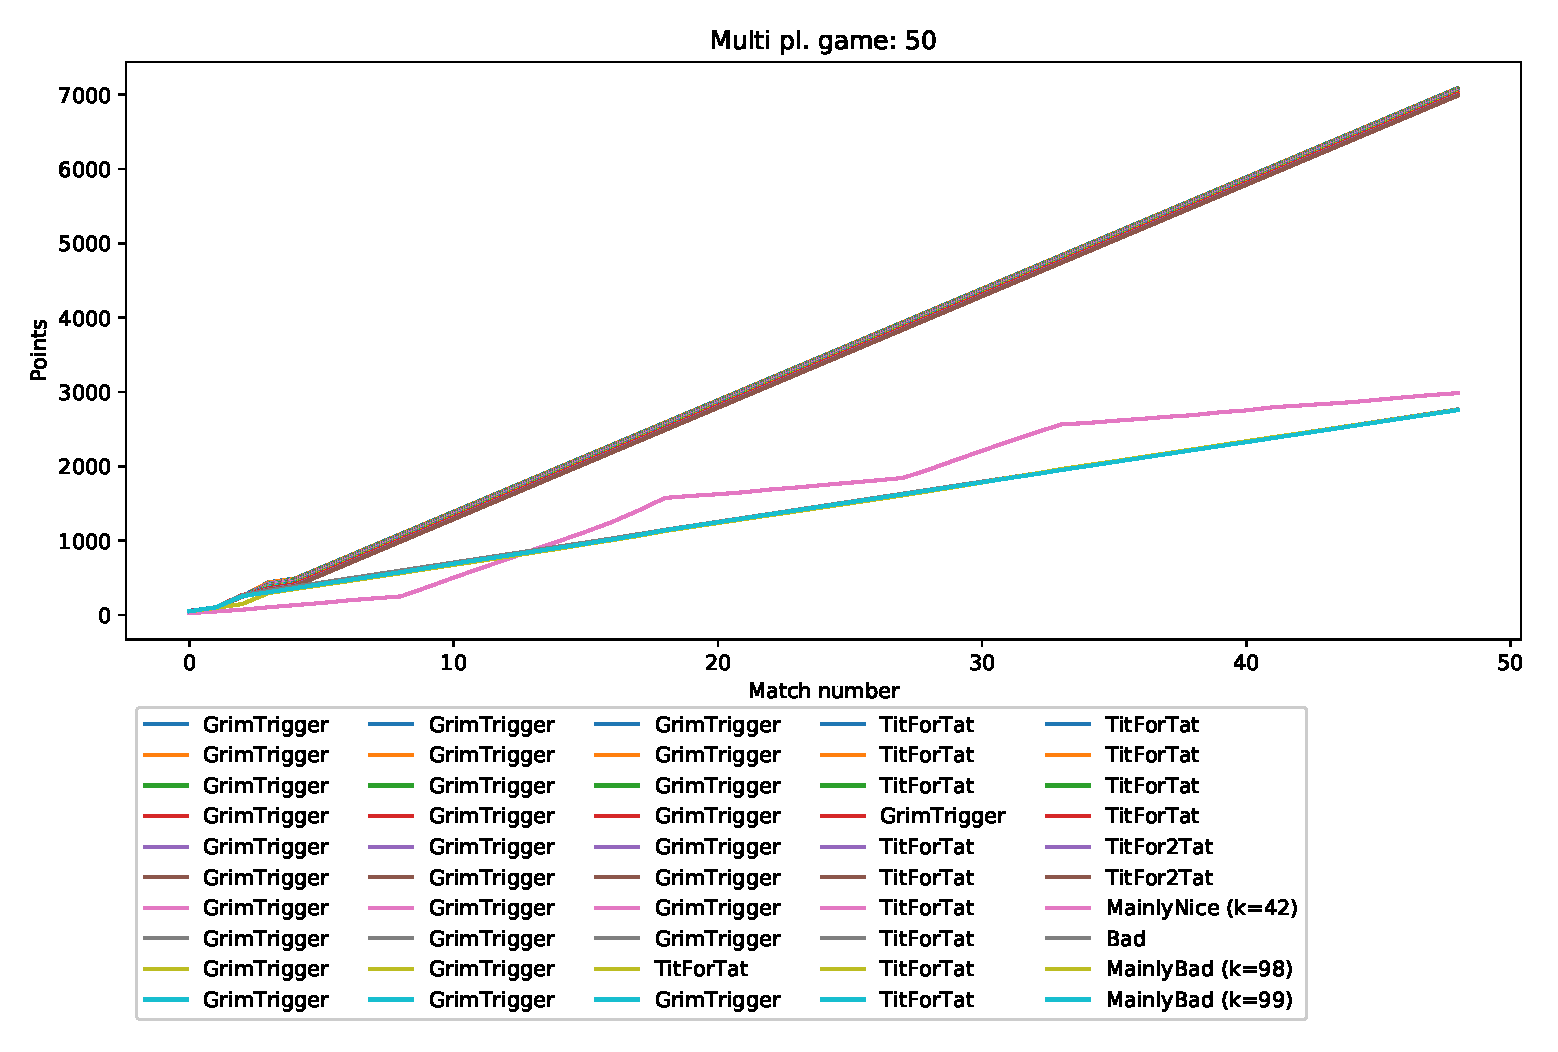
\includegraphics[width=1\columnwidth]{../img/ripdmp-const/ripdmp-scores-const-pop-50-r3}
    \caption{Last iteration scores ($it=3$)}
    \label{fig:constLI}
\end{figure}

\begin{table*}[ht]
    \caption{rMPIPD, constant pop, strategy evolution \textbf{TODO IF NOT FIXED, USE TRANSPOSE (2 cols missing)}}
    \label{tab:ripdmp-const}
    \centering
    \begin{tabular}{c|rrrrrrrrrrrrrrrrr} \toprule
        iter & GrT & Tf2T & TfT & Nice & MN (3) & MN (8) & MN (17) & MN (42) & Ind & MB (70) & MB (78) & MB (81) & MB (85) & MB (97) & MB (98) & MB (99) & Bad \\ \midrule
        1 &  5 &  7 &   8 &  6 &  1 &  1 &  1 &  1 &  7 &  1 &  1 &  2 &  1 &  1 &  1 &  1 &  5 \\
        2 &  5 &  7 &   8 &  6 &  1 &  1 &  1 &  1 &  7 &  1 &  1 &  2 &  1 &  1 &  1 &  1 &  5 \\
        3 &  4 &  6 &  15 &  3 &  1 &  0 &  0 &  1 &  3 &  1 &  2 &  3 &  1 &  1 &  2 &  1 &  6 \\
        4 &  3 &  4 &  28 &  0 &  0 &  0 &  0 &  1 &  0 &  1 &  1 &  3 &  1 &  1 &  2 &  1 &  4 \\
        5 &  1 &  2 &  36 &  0 &  0 &  0 &  0 &  1 &  0 &  1 &  1 &  2 &  1 &  0 &  2 &  1 &  2 \\ \bottomrule
    \end{tabular}
\end{table*}

\subsection{Increasing Population}
In this case the number of players (population) is increased at each iteration. We implemented three different way of modifying the population between rounds; after each round a player has a certain probability based on his ranking to have a child of the same type:
\begin{enumerate}
    \item The probability is $p(i)=1- i\ /\ num\_players$ where $i$ is the position reached by the player. The winner of the round is indeed doubled, because $p(0)=1$, while the looser is not, as $p(last)=0$.
    For each player we draw a random number, accordingly to a uniform probability distribution, and compare it with $p(i)$, if it is greater we effectively double it, otherwise we do not.
    \item We draw a random number $d$ and split the rank-ordered population in three sets of equal size $A,B,C$. The player is doubled if:
    \begin{itemize}
        \item $d>0.2$ if the player belongs to $A$
        \item $d>0.5$ if the player belongs to $B$
        \item $d>0.8$ if the player belongs to $C$
    \end{itemize}
    This is an alternative way to promote best strategies and obstruct less performant players.
    \item We define a player's score as its obtained points divided by the maximum obtained score in the whole population. We double the player if a drawn random number is greater than its score.
\end{enumerate}

We used by default the first of the three proposed methods, but the method may be statically set using the \texttt{ALTERNATIVE} variable.

Figures~[\ref{fig:incrR},\ref{fig:incrFI},\ref{fig:incrMI},\ref{fig:incrLI}] show the evolution of a population of 50 players over four iteration. In this case we do not have convergence at the fifth iteration, since the population is increasing, but the simulation still exhibits the same behaviour. The \textit{TfT} strategy is getting stronger and stronger. It is concluded that, in the future, i.e. evaluating the problem with more iterations, the population will increase with similar behaviour and converge to the \textit{TfT} strategy.

\begin{figure}[!ht]
    \centering
    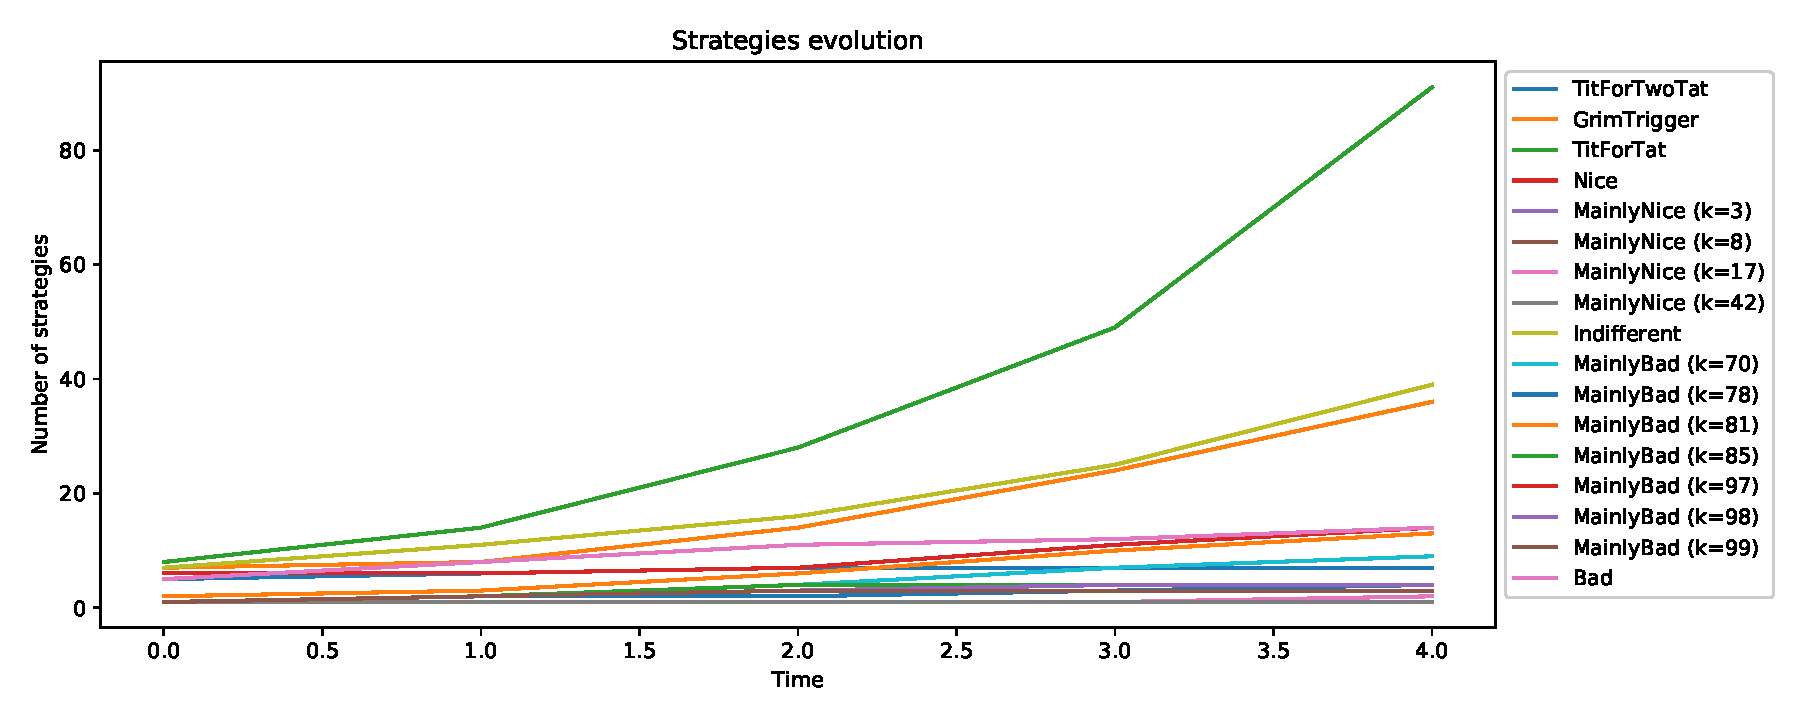
\includegraphics[width=1\columnwidth]{../img/ripdmp-incr/ripdmp-evolution-increasing-pop-50}
    \caption{Evolution of rIPDMP, increasing population of 50}
    \label{fig:incrR}
\end{figure}

\begin{figure}[!ht]
    \centering
    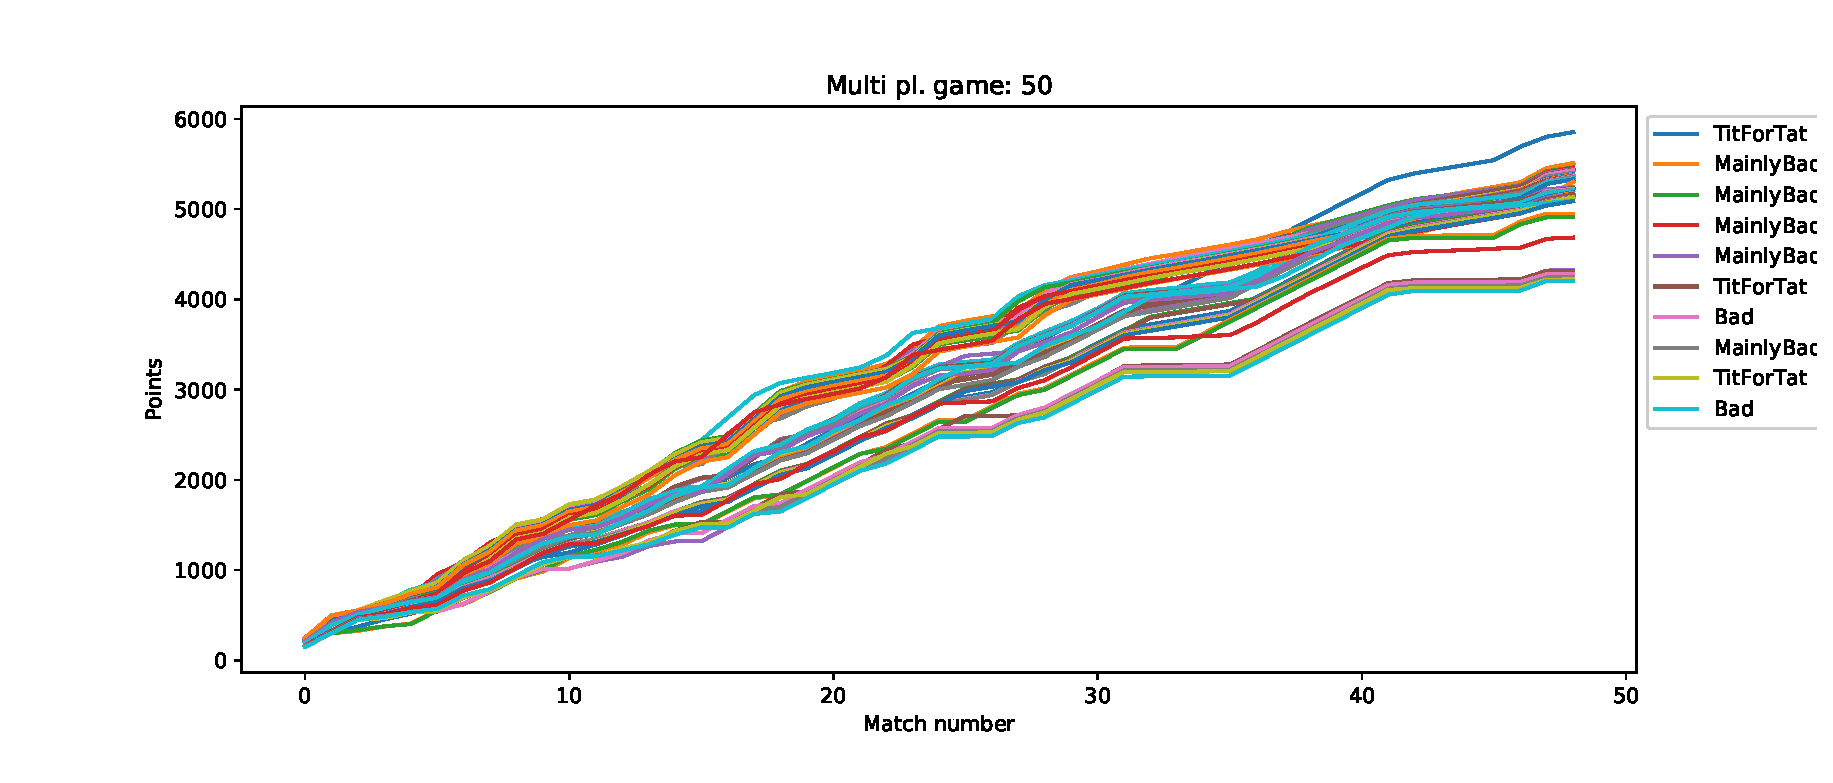
\includegraphics[width=1\columnwidth]{../img/ripdmp-incr/ripdmp-scores-increasing-pop-50-r0}
    \caption{First iteration scores ($it=0$)}
    \label{fig:incrFI}
\end{figure}

\begin{figure}[!ht]
    \centering
    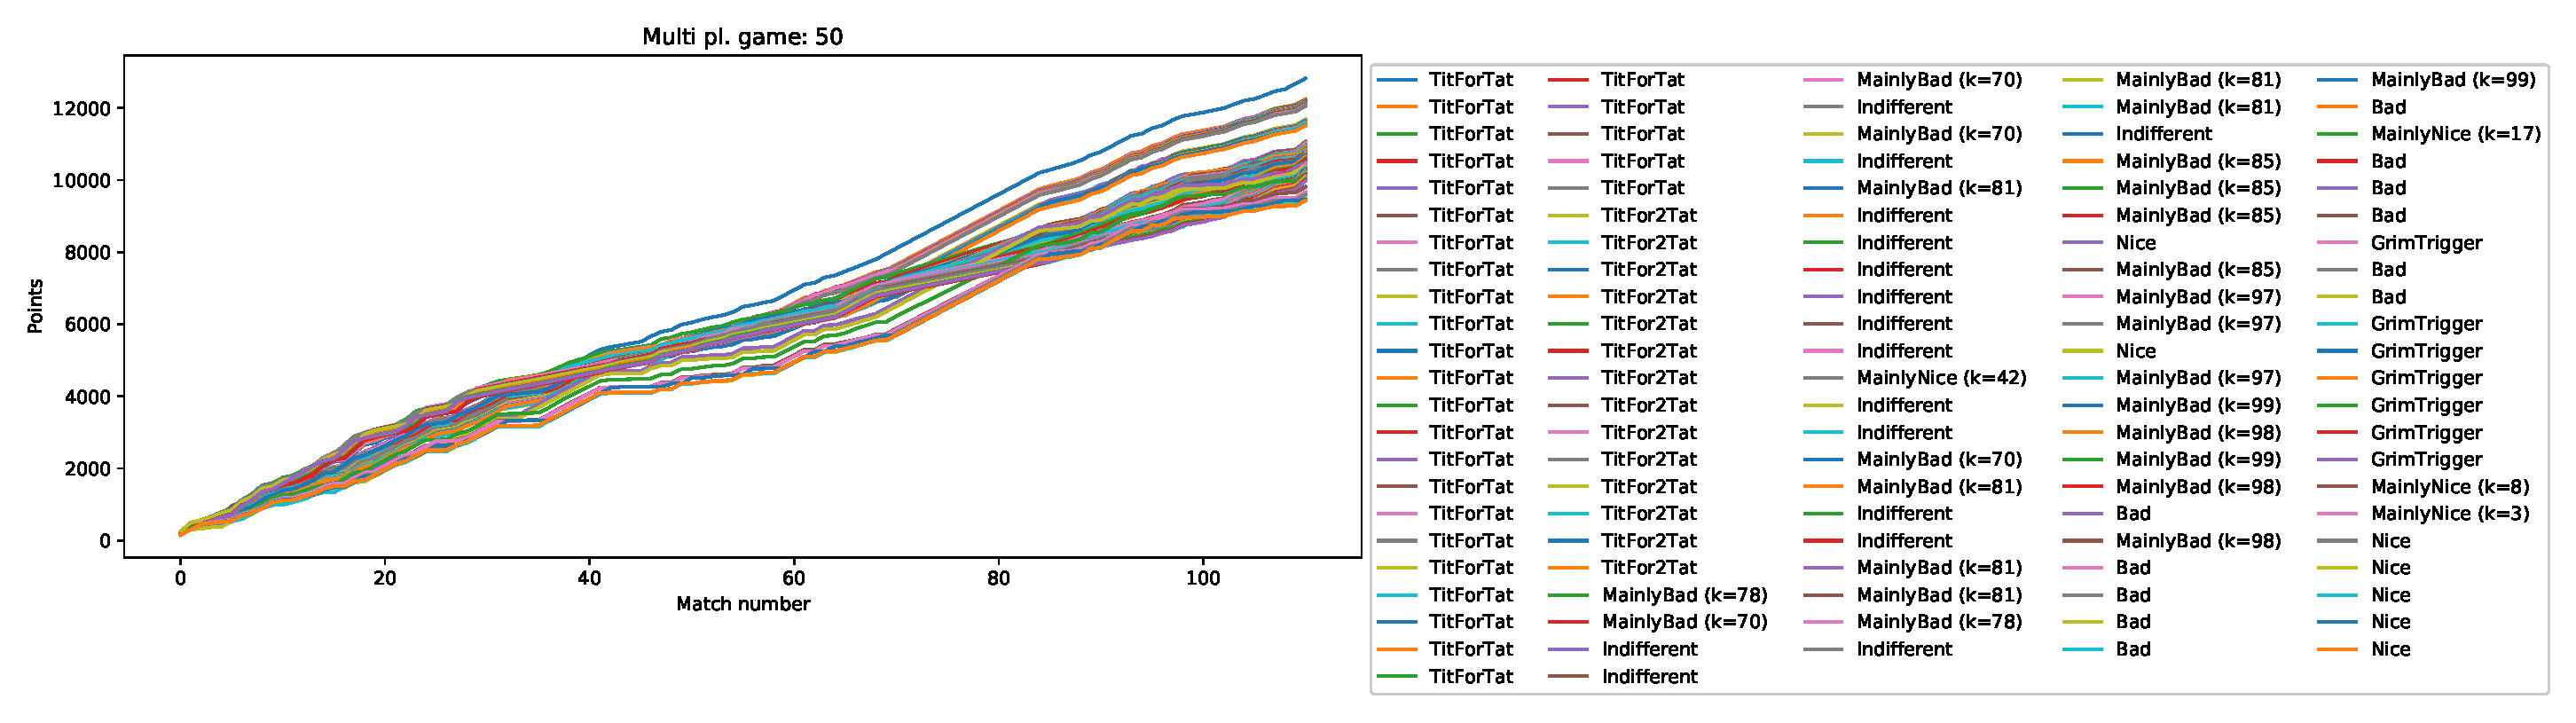
\includegraphics[width=1\columnwidth]{../img/ripdmp-incr/ripdmp-scores-increasing-pop-50-r2}
    \caption{Middle iteration scores ($it=2$)}
    \label{fig:incrMI}
\end{figure}

\begin{figure}[!ht]
    \centering
    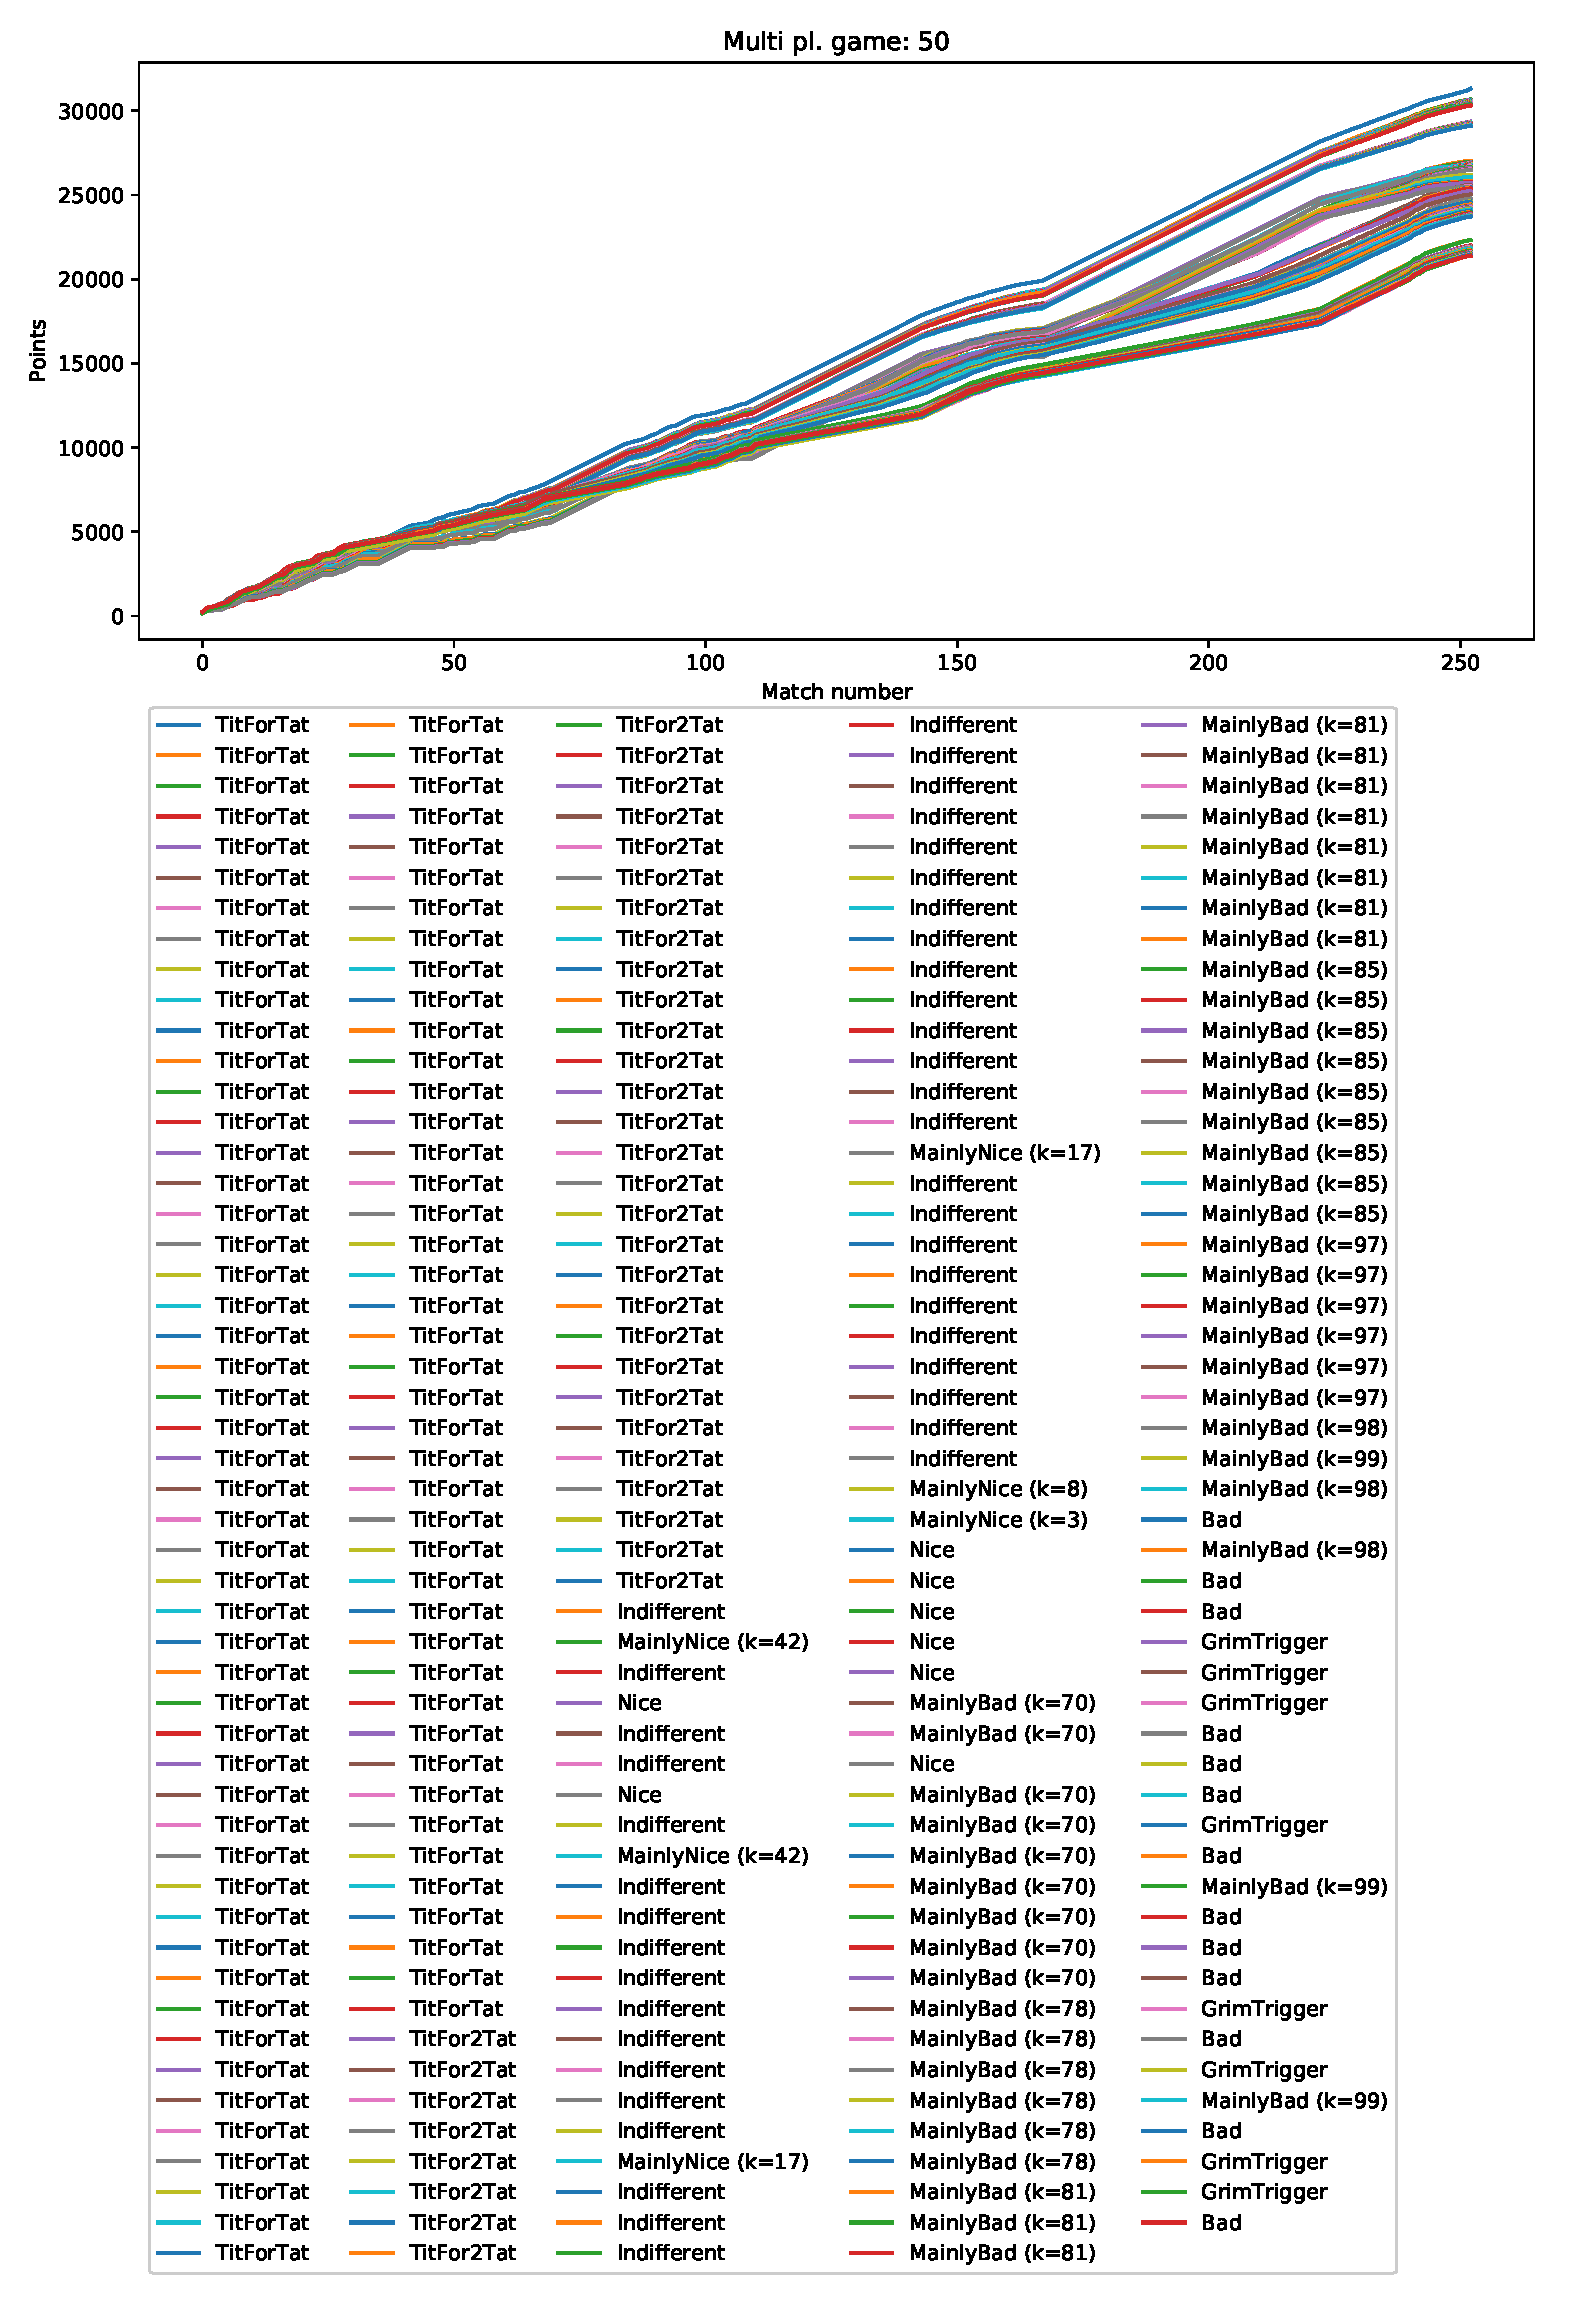
\includegraphics[width=1\columnwidth]{../img/ripdmp-incr/ripdmp-scores-increasing-pop-50-r4}
    \caption{Last iteration scores ($it=4$)}
    \label{fig:incrLI}
\end{figure}

\begin{table}[ht]
    \caption{rMPIPD, increasing pop, strategy evolution\\ \textbf{TODO OR BOTH FIXED OR BOTH FREE}}
    \label{tab:ripdmp-const}
    \centering
    \begin{tabular}{c|cccccccc} \toprule
        iter & GrT & Tf2T & TfT & Nice & MN (25) & Ind & MB (75) & Bad \\ \midrule
        1 &   1 &   1 &   1 &  1 &  1 &  1 &   1 &   1 \\
        2 &   2 &   2 &   2 &  1 &  2 &  2 &   2 &   2 \\
        3 &   4 &   2 &   3 &  1 &  2 &  3 &   3 &   4 \\
        4 &   7 &   3 &   5 &  1 &  3 &  3 &   5 &   7 \\
        5 &  12 &   3 &   9 &  1 &  3 &  3 &   6 &  12 \\
        6 &  16 &   3 &  17 &  1 &  3 &  3 &   8 &  18 \\
        7 &  19 &   5 &  33 &  1 &  3 &  3 &  15 &  27 \\
        8 &  19 &  10 &  62 &  1 &  6 &  5 &  23 &  33 \\ \bottomrule
    \end{tabular}
\end{table}

It is interesting to note how Wu and Axelrod~\cite{IPDnoise} exploit this behaviour to react to noise in the game: just by slightly altering the \textit{TfT} strategy in both directions, adding generosity (some percentage of opponent's defections go unpunished) or contrition (avoid responding to a defect move when a player's previous defection was unintended) the ``error'' can be quickly recovered and cooperation can be successfully restored. Note however that we do not implement these two variations of the \textit{TfT} strategy in this work.

\section{Changing rMPIPD - RR scheme} \label{s:crIPDMP}
We finally also made another step further by allowing players to change their strategies in the rIPDMP setup, of which the main structure is unaltered. The change of strategy is again based on players' ranking: a strategy that gives good results is enhanced and a bad strategy leads to a change towards the ``opposite'' direction.
\textbf{Left loose on purpose because of the todo in change_strategy calling for review. Will be more detailed}

\section{Adding Machine Learning}
\textbf{ADD THIS IN THE INTRODUCTION}
Since the birth of this subject studies have been developed to help us find an insight that may be lay under the problem, some pattern that we could not figure out. \textbf{CITE PAPER FROM 60s}

Moreover, neural networks and artificial intelligence techniques can also be used to tackle this problem: for examples on the use of reinforcement learning approaches we refer the reader to \cite{sandholmRL,plosRLdominant,coopSeqRL,kedaoRL} and to \cite{shashiEvoAlg} for an example using evolutionary algorithms.

\textbf{Go on}


\section{Conclusions} \label{s:conc}
\textbf{TODO some conclusion to blend with introduction}
This work can easily be extended in many ways in a future development: for example, a lot of new and more complex strategies were created since the original tournaments made by Axelrod and these may be incorporated in the analysis aside of the present ones.
Moreover, we could try to investigate further in getting a good metric to use with reinforcement learning. \textbf{rewrite after paper reading}

\textbf{THIS IS PASTED FROM A WEBSITE REWRITE!!!}
When paired with a mindless strategy like RANDOM, TIT FOR TAT sinks to its opponent's level. For that reason, TIT FOR TAT cannot be called a ``best'' strategy.
\textbf{TfT non punta a vincere le battaglie ma la guerra}

It must be realized that there really is no ``best'' strategy for prisoner's dilemma. Each individual strategy will work best when matched against a ``worst'' strategy. In order to win, a player must figure out his opponent's strategy and then pick a strategy that is best suited for the situation.

\balance
\bibliographystyle{IEEEtran}
\bibliography{report}
\end{document}
